\documentclass{article}
\setlength{\parskip}{0.67\baselineskip}
\usepackage[a4paper, total={6in, 8in}]{geometry}
\usepackage{graphicx}
\usepackage{listings}
\usepackage{xcolor}
\usepackage{float}
\usepackage{fancyhdr}
\usepackage[utf8]{inputenc}


\pagestyle{fancy}
\fancyhf{}

\lhead{Max Stupple - A-Level Computer Science Project}
\rhead{\thepage / \pageref{page:the_end}}

\title{A-Level Computer Science Project\\ Task Scheduler}
\author{Max Stupple}
\date{}

\lstset{
	frame=tb, % draw a frame at the top and bottom of the code block
	tabsize=4, % tab space width
	showstringspaces=false, % don't mark spaces in strings
	numbers=left, % display line numbers on the left
	basicstyle=\small,
	commentstyle=\color{gray}, % comment color
	keywordstyle=\color{blue}, % keyword color
	stringstyle=\color{red}, % string color
	breaklines=true, % allow line wrapping
}

\begin{document}

\pagenumbering{gobble}
\maketitle
\pagebreak

\pagenumbering{arabic}
\tableofcontents
\pagebreak

\part{Analysis}
\section{Overview of the problem}
Many students struggle to manage their time. The workload of A-levels alone is
enough to make it difficult to balance between small pieces that are due in
soon, and longer projects which need to be worked on frequently; let
alone extra-curricular activities and sports that take up more time after school
and on weekends. One solution is to manually plan how you will use all your free
time, but this has two drawbacks:

\begin{samepage}
	\begin{itemize}
		\item Many people struggle to estimate how long a task will take them and hence
		      struggle to allocate a reasonable amount of time to each task
		\item This process takes time, a resource which has already been established to
		      be finite and valuable
	\end{itemize}
\end{samepage}

My stakeholder (henceforth referred to as SH) is a Sixth Form student
studying Maths, Further Maths, Physics and Chemistry. He struggles to fit in all
his work around his various extra-curricular activities, so he needs an app that
will not only help him keep track of what he needs to do, but timetable when to do each task and prioritise those which are most urgent. SH represents the needs
of my target user group.

\section{Limitations of current system}
To organise his tasks, SH currently uses the Apple Reminders app on his iPhone.
However, he finds this lacking for a number of reasons. Although the app helps
him keep track of the tasks he needs complete and when they are due, it does not
help him prioritise these tasks or inform him of the relationship between the
amount of time he needs to do those tasks and the amount of time he has before
they are due. He also doesn't find the app very engaging, as he lacks a sense of
accomplishment after completing a task and ticking it off his list. Furthermore,
the app only provides the ability to sync between Apple devices, which he finds
limiting as he cannot access his tasks on his Windows computer.

\section{Initial ideas}
This initial feature list will help me research existing software which may
partially solve the problem. It will also give an idea of how complex the final
solution will be.

To satisfy the needs of SH, I anticipate a solution will need to fulfil the
following functions:

\begin{samepage}
	\begin{itemize}
		\item Keep a list of the users tasks which contain a description of the task, a
		      due date and time estimate
		\item Schedule tasks in user's free time according to a calendar and school/work
		      schedule
		\item Record and track the actual time taken to complete a task, including
		      breaks
		\item Provide feedback on the accuracy of the user's time estimates and
		      productivity levels
		\item Adapt to the user's preference in terms of length of work sessions
		\item Display these tasks to the user is an organised manner using a Graphical
		      User Interface
	\end{itemize}
\end{samepage}

The program will be created as a web app using the Django web framework. The
reason for creating it as a web app is so that it is available as widely as
possible, as it will be possible to access it on any device with a modern web
browser. Django will allow me to deploy my solution in a modern and efficient
way, so that I can focus on the underlying data structures, while Django mostly
handles the interface. The data structures will also be implemented using Python
in an object-oriented way, which I think is sensible as this is a tool which I'm familiar
with working with.

\section{User group}
My target users are students, in particular Sixth Form and University. As the
program is targeted at individuals who struggle to manage their time and avoid
procrastination, the program will need to be engaging and provide incentives for
the user to complete tasks early rather than delaying them. Thus the user will
avoid situations in which they find themselves with insufficient time to
complete all their tasks before they are due.

The UI must also be simple and intuitive to use: there's no point in using an
app to organise your time if you waste more time trying to get the app to work
than doing the work you need to do.

\section{Computational methods}
This problem lends itself to a computational solution in particular due to the
need for automation and interactivity to ensure engagement. One potential
non-computational solution could be a physical calendar or to-do list, however
this would not be able to provide the features required by my client. Such a
solution could not automatically allocate time for the user to complete their
tasks in, and could not remind the user of their tasks - it would require the
user to check and plan the time for themselves.

\subsection{Abstraction}
Data will be stored with an object-oriented approach. Tasks, events, routine
events, and allocated time slots will all be objects with appropriate
relationships so that the data can be viewed from a number of perspectives.

\subsection{Reusability}
There are a number of functions which my program will need to perform where it
wouldn't make sense to write them myself from scratch, so I will use libraries
that have already solved the problem. I will need to be able to get the current
date and time, to associate with each task, and a SQL database to store my data
in.

\subsection{Visualisation}
My program will need to be able to present data to the user in a way that is
visually appealing and easy to understand. For example, data about the number of
tasks completed can be presented on a histogram.

\subsection{Concurrency}
The program will need to be able to perform certain tasks in the background
without interrupting the user, for example allocating time slots to tasks and
analysing data to create graphs and provide feedback to the user.

\subsection{Data Mining}
Albeit on a small scale, my program will use the concept of data mining to
analyse trends in the user's completion of tasks, such as how much time they
spend and how accurate their time estimates are, in order to give feedback and
help the user improve their efficiency.

\subsection{Logic}
The program will need to be able to intelligently allocate time slots to tasks
based on the user's schedule and the time needed to complete the task. It will
also need to be able to adapt the user's habits and preferences regarding their
work schedule.

\section{Research}
I identified a number of candidates for solutions to SH's problem. The candidate
programs are:

\begin{samepage}
	\begin{itemize}
		\item Forest
		\item Evernote
		\item Todoist
		\item Remember the Milk
		\item Ike
		\item Google Keep
		\item Trello
	\end{itemize}
\end{samepage}

\begin{figure}[h]
	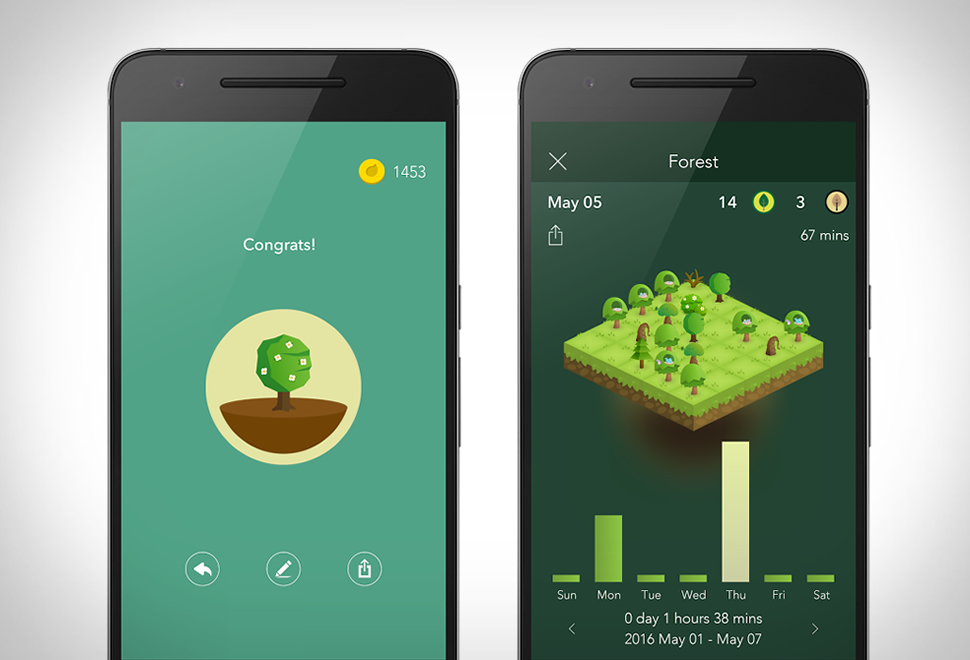
\includegraphics[width=\linewidth]{Images/forest.jpg}
	\caption{Forest}
	\label{fig:forest1}
\end{figure}

Forest is the only candidate dedicated to helping the user focus on their tasks
and get stuff done as quickly as possible by avoiding distractions. It's primary
feature is an animated forest which grows as you work, but dies if you leave the
app. This encourages the user to avoid 'quickly' having a look at Facebook,
sending a text or otherwise breaking their workflow. Forest shows you how much
time you spent each day growing your forest, so you can see which days you were
most productive on. The primary drawback of Forest is that it lacks any means of
tracking tasks from within the app. In my view this is significantly problematic
as the app which is going to help you focus the most is one which never needs
you to leave while working. Integrated task management is an
absolute must for my solution.

\begin{figure}[h]
	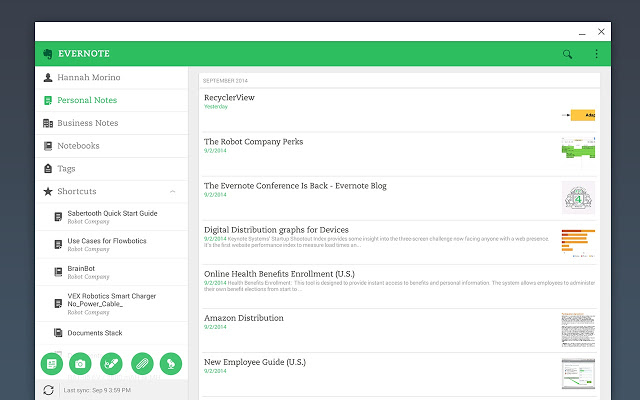
\includegraphics[width=\linewidth]{Images/evernote.jpg}
	\caption{Evernote}
	\label{fig:evernote1}
\end{figure}

Evernote is primarily focused on note-taking, organisation and task-management.
The power of it's note-taking is remarkable, and can include voice memos,
handwritten notes and embedded web pages. However, most of these features are
superfluous for my product, and would needlessly add complexity.

\begin{figure}[h]
	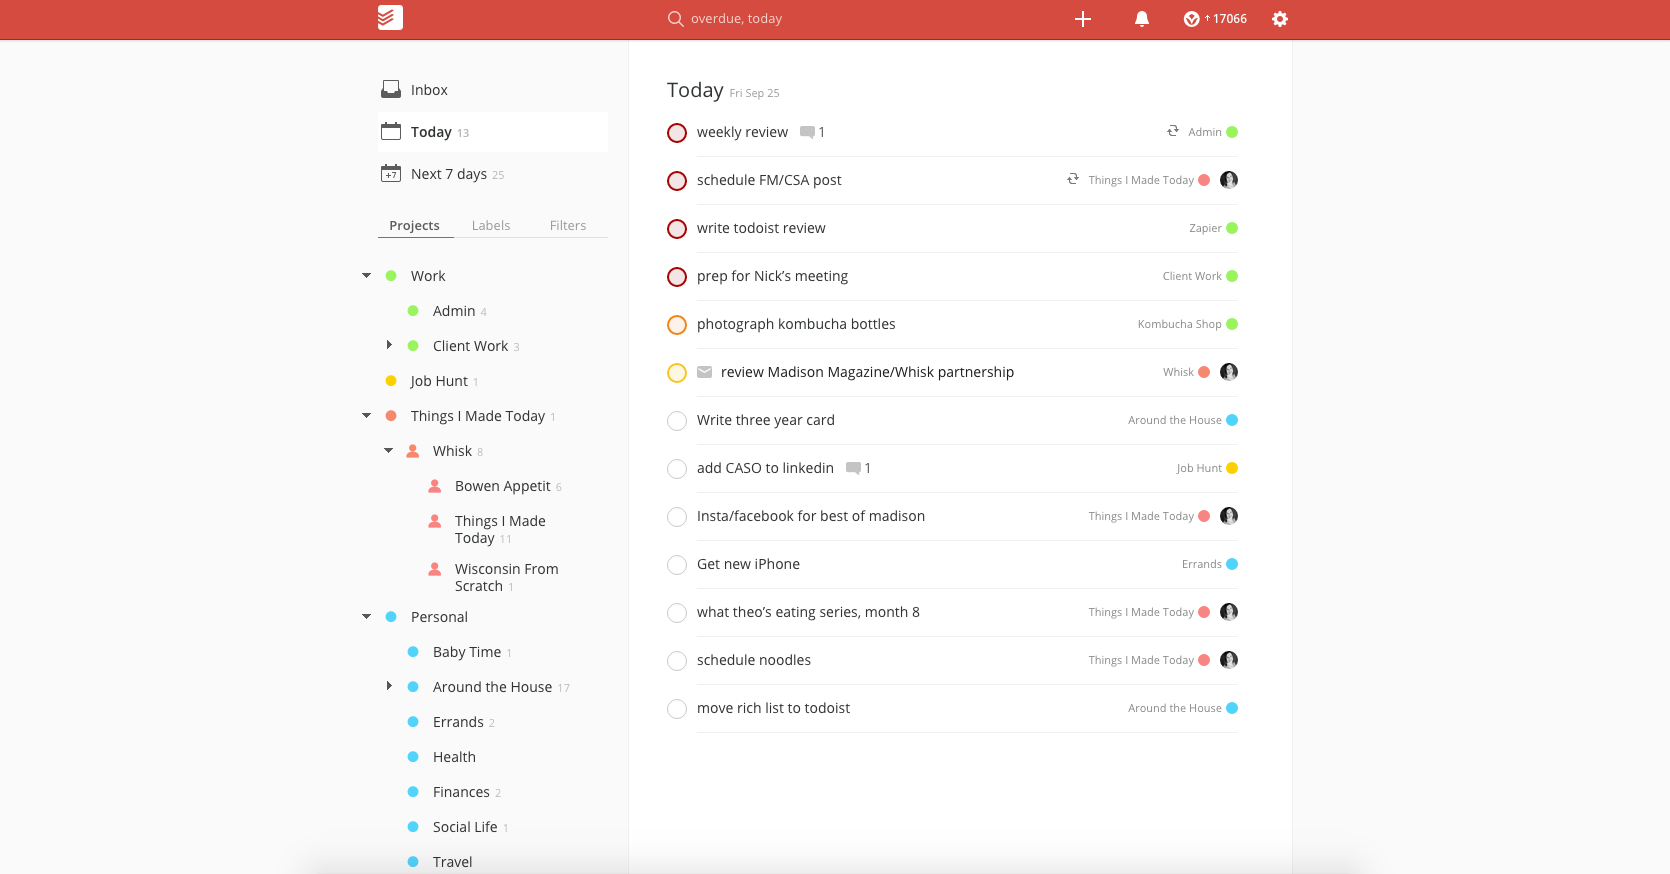
\includegraphics[width=\linewidth]{Images/todoist.png}
	\caption{Todoist}
	\label{fig:todoist1}
\end{figure}

Todoist is the only of these apps which is laser-focused on to-dos. One of its
prominent features is the ability to write tasks in natural language, which it
then understands when they are due, if they are recurring etc. This is beyond
the scope of my product, however I am interested in the tools they have for
tracking your productivity. Todoist can display graphs of total number of tasks
done per day/week, the distribution between different types of tasks e.g.
whether you did more tasks tagged with ``Study'' or ``Chores''. I definitely
want to have similar visualisations of how productive the user is being.

\begin{figure}[h]
	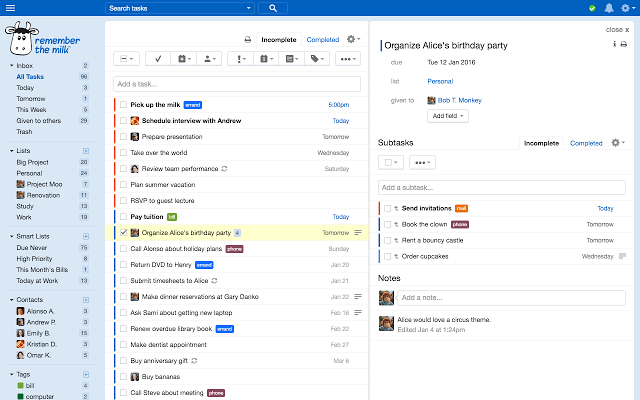
\includegraphics[width=\linewidth]{Images/remember-the-milk.png}
	\caption{Remember The Milk}
	\label{fig:rtm1}
\end{figure}

Similar to Todoist, Remember the Milk has a lot of advanced tools for
intelligently adding, sorting and searching through tasks. However I'm
particularly interested in the ability to divide tasks into sub-tasks. I
personally have used to-do apps with such a feature and have found it rather
useful, so I'll be interested to get my stakeholder's opinion on this
feature specifically when I talk to them.

\begin{figure}[h]
	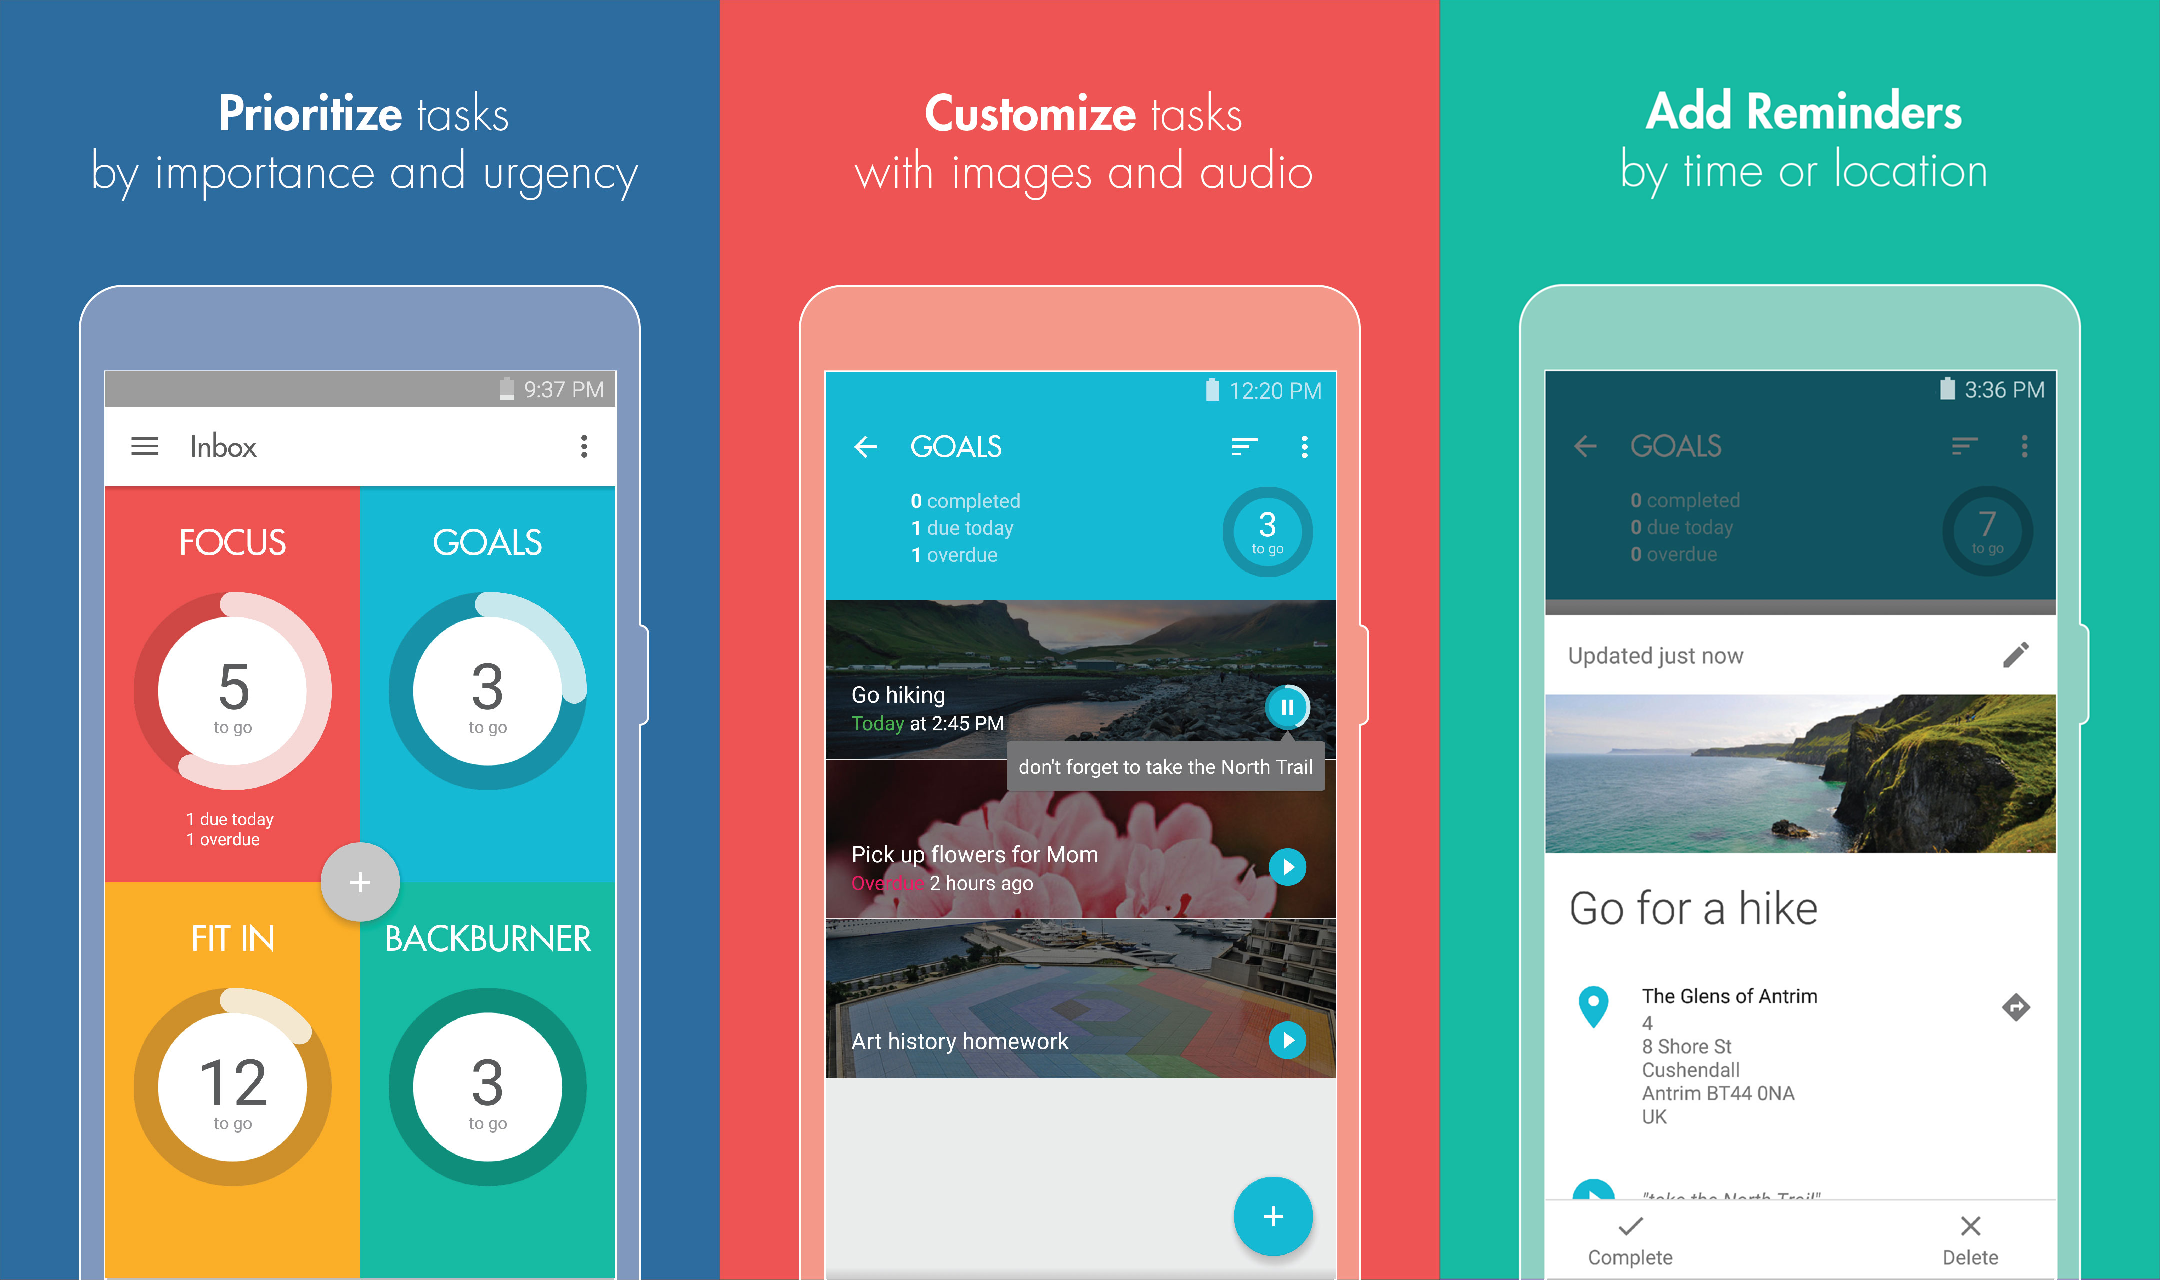
\includegraphics[width=\linewidth]{Images/ike.png}
	\caption{Ike}
	\label{fig:ike1}
\end{figure}

Ike is in fact the to-do app which I currently use. I can't say that I'm
entirely satisfied with it, but I like the system of organising tasks into
``Urgent and Important'', ``Urgent but not Important'', ``Important but not
Urgent'' and ``Neither Urgent nor Important''. I think this is a useful system
and could perhaps be preset in my product, but I find it limiting that Ike
forces you to organise by those categories. I definitely want my product to
allow the user to organise their tasks into whatever folders and sub-folders
they please. I think any limitation on how the tasks are organised will always
be counterproductive in some degree to some users.

\begin{figure}[h]
	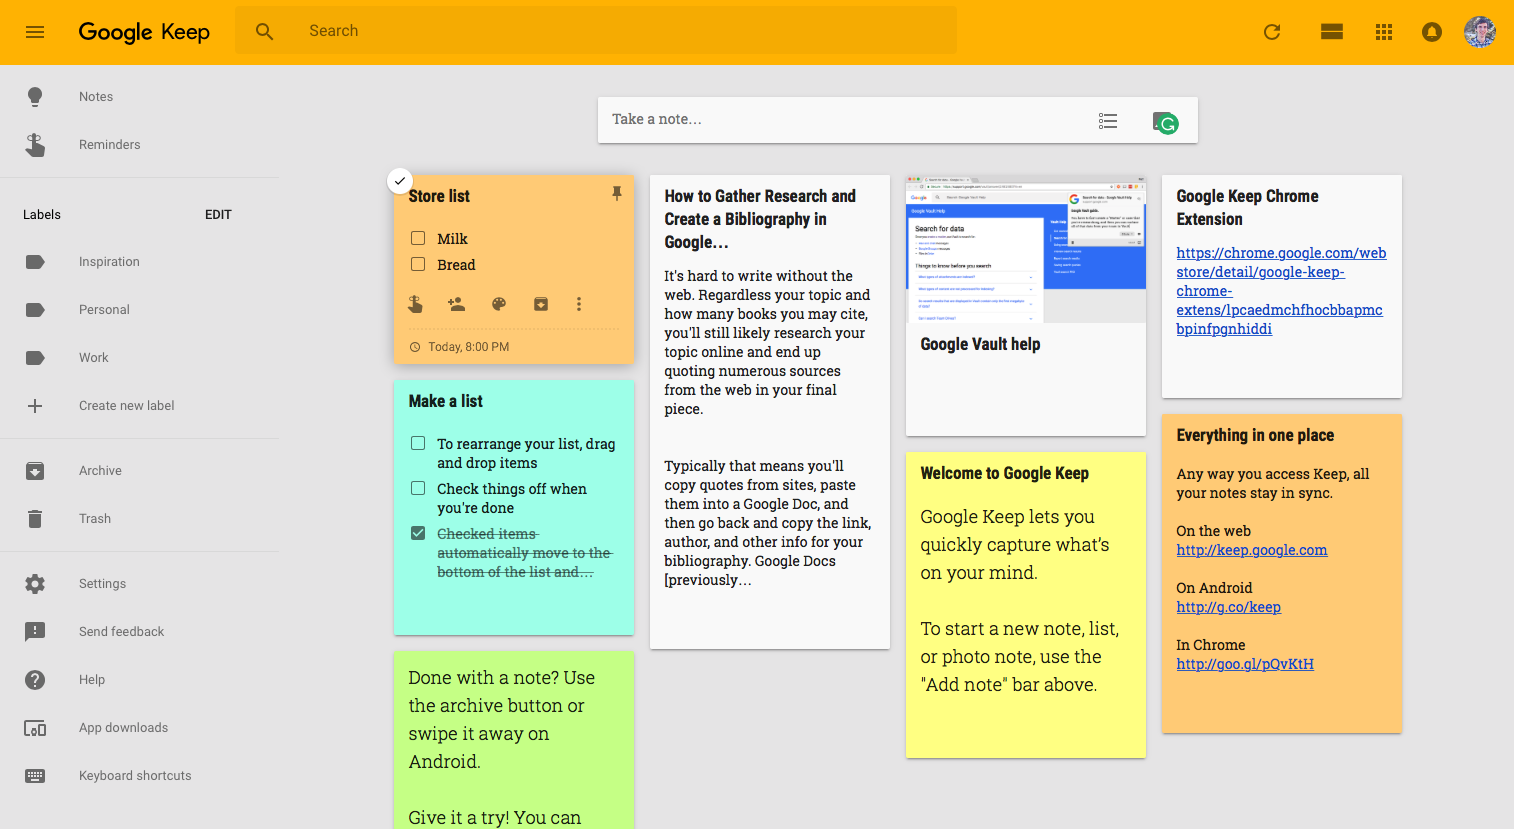
\includegraphics[width=\linewidth]{Images/keep.png}
	\caption{Google Keep}
	\label{fig:keep1}
\end{figure}

Keep is quite a good, basic to-do app. Keep's main interesting feature is its
integration with the rest of Google's ecosystem, however this isn't really
something that my project is too concerned with. I'm also not a fan of Keep's
visual metaphor of tasks being ``cards'' on the screen - a common visual
metaphor in Google's design language. I think this creates confusion as there is
not simply a vertical list. I also dislike that you need to create different
types of tasks for simple text, lists, voice memos etc.

\begin{figure}[h]
	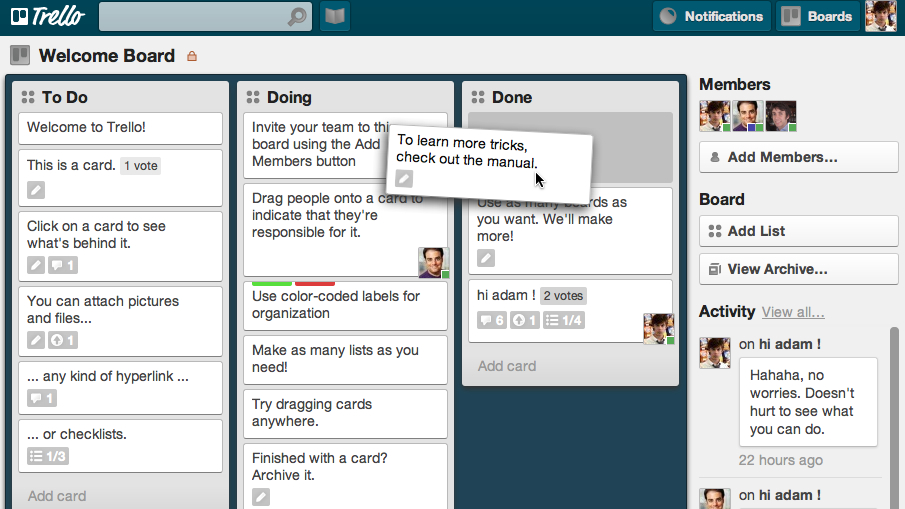
\includegraphics[width=\linewidth]{Images/trello.jpg}
	\caption{Trello}
	\label{fig:trello1}
\end{figure}

Trello is more focused on managing multi-person projects than an individual's
todo list. It's most prominent feature is the ability to work collaboratively on
creating tasks, marking them complete, adding comments and so on. However I
think this sort of feature is beyond the scope of my solution. However I do like
that each ``card'' can - unlike Keep - have text, checklists, and attachments. I
think it will be useful for my users to be able to attach a reasonable amount of
information to their tasks.

I think these programs all offer partial solutions to the problem, but none of
them offer a solution to the exact problem SH has described. Forest is excellent
for helping you focus on a task, but can't keep track of your to-dos. Todoist
offers excellent functionality for keeping track of and organising your tasks,
but doesn't do anything with regard to helping you timetable everything that you
need to do. Keep is better in this regard as it integrates with GCal to display
tasks in your calendar, but can't allocate them those time slots automatically.
Ike has a very appealing UI and a good system for organising into four
overarching categories, but you can't create your own categories like Todoist.
Remember the Milk is probably the most intelligent of the programs, with a
``Smart Add'' feature that makes adding tasks very simple, and a powerful search
for filtering through your tasks, in addition to integrating with a number of
other services such as email and social media for reminders, and cloud storage
services for adding attachments to tasks, however this is probably beyond the
scope of the problem I'm trying to solve. Evernote is in my opinion the least
effective of these programs, as it is mainly focused on note taking, with
reminders as a side-feature. Trello offers the most features oriented towards
time management and prioritising tasks, but is more focused around team
collaboration on big projects than individual to-do management.

I showed the candidates to SH to get his opinion and he gave me the following
comments:

\begin{description}
	\item Forest: ``This is my favourite. The UI is excellent and the metaphor of
	      growing trees is very appealing. Out of all the programs this does the best
	      job of helping me manage my time, however it's unfortunate that is doesn't
	      include integrated task management. I like that you can see your past progress
	      as this is very motivational, and it stops the timer if you leave the app,
	      which helps you avoid idly switching to Facebook or Twitter for a 'quick
	      check'.''
	\item Evernote: ``Good for note taking, but that's not really what I'm looking
	      for. It has too many extraneous features, which are unnecessary and make it
	      feel bloated - I want a more streamlined experience. I also dislike the
	      subscription model.''
	\item Todoist: ``Great for managing tasks, with graphs and data to track your
	      statistics. I love the categorisation and colour coding for different tasks,
	      and being able to give them different levels of priority. I also like that you
	      can export your tasks to your calendar. The lack of a dark mode harms the
	      UX.''
	\item Remember the Milk: ``There's too much task segregation which makes the UI
	      confusing. It also has a weird notes system. Not a fan.''
	\item Ike: ``The idea behind it is admirable, but ultimately the categories feel
	      a bit arbitrary, and that's made worse by the lack of an 'all tasks' view. The
	      UI is very clean however, and the animations are really nice.''
	\item Keep: ``It's good for lists, but otherwise nothing special.''
	\item Trello: ``Good for project development, but not well-suited to personal
	      task management.''
\end{description}

He also commented in general that he liked the ability to sync tasks between
devices, and a feature which he wanted but none of the programs offered was the
ability to have ``subtasks'' nestled inside other tasks.

\subsection{Features of the proposed solution}
From this I have assembled the following list of features which my program will
need:

\begin{samepage}
	\begin{itemize}
		\item Main view displays all uncompleted tasks and recently completed but
		      not-deleted tasks
		\item Archive containing completed tasks, and allows tasks to be un-marked as
		      complete
		\item Tasks grouped in categories
		\item Tasks can be filtered by category
		\item Ordered by time needed or due date
		\item Tasks can be marked as done or deleted
		\item New tasks can be added, with a brief title, optional additional notes, an
		      estimate of time needed and a due date
		\item Graphs showing number of tasks completed, amount of time taken, and
		      whether tasks were completed on time
		\item Show upcoming tasks in their automatically allocated time slots
		\item User can enter the schedule and other commitments that the program will
		      schedule tasks around
		\item The program will give a warning if there is not enough free time to
		      complete a given task before it's due date
		\item Current task displayed at top of screen
		\item Time spent working and time to next break
		\item Buttons to manually pause timer and take a break or mark task as done
		\item Graphic showing a town/city building up over time as you work
	\end{itemize}
\end{samepage}

I showed this list to SH, and he added that tasks should be given a priority
level, so that high priority tasks can be scheduled before low priority ones. He
also elaborated on the city-building mechanic, resulting in the following:

\begin{samepage}
	\begin{itemize}
		\item The city builds over time as you work
		\item Taking a break which has been allocated by the app simply pauses

		\item Taking an unallocated break sets the development back - perhaps there is a
		      level system and you can be set back one or two levels
		\item If you quit a task before you finished - and taking an excessively long
		      break automatically quits - the city is destroyed
		\item If you take too long to complete a task, development is slowed down
		\item When you finish a task, you can either stop, which doesn't destroy your
		      city but it degrades over time, or go straight to the next task, in which case
		      progress continues
		\item If you finish a task early and go straight on to another task, your city
		      gets a boost
	\end{itemize}
\end{samepage}

SH said he ``agrees with all of this'' and called it ``good design''. He also
emphasised his desire to access his tasks across different devices. I have
concluded that the best way to facilitate this would be to build the program as
a web app. This is the easiest way to make it available cross-platform, as it
should be accessible on any device with a modern web browser.

SH also suggested that there were psychological benefits to offering the user a
choice in what task they do. Studies have shown that individuals are more
motivated to complete a task which they have chosen to do from a set of options,
rather than only one. Therefore I will endeavour to implement a system which,
rather than forcing, or heavily encouraging, the user to complete one particular
task in a certain time slot, will instead give them the option to choose between
tasks with similar levels of priority.

\subsection{Limitations of the proposed solution}
The main way in which my solution will be limited,
compared to those products researched,
will be the inability to sync to an external calendar,
as for example Google Keep can.
Users might like to sync their events from their existing calendaring solutions,
but I think implementing such a feature is beyond my project's scope.

It will also be limited in the depth of the task management,
when compared to a product such as Todoist.
I won't include features such as organising tasks into ``projects'',
or collaborating on tasks,
as this would greatly increase complexity,
and again,
it really beyond the scope of the problem I am aiming to solve.


\section{System requirements}
As the program will be web-based, it will require a system capable of running a
modern internet browser, such as Firefox. The system requirements for Firefox
66.0 are as follows:

\subsection*{Windows}\label{windows}

\subsubsection*{Operating Systems (32-bit and
	64-bit)}\label{operating-systems-32-bit-and-64-bit}

\begin{samepage}
	\begin{itemize}
		\item Windows 7
		\item Windows 8
		\item Windows 10
	\end{itemize}
\end{samepage}

\subsubsection*{Recommended Hardware}\label{recommended-hardware}

\begin{samepage}
	\begin{itemize}
		\item Pentium 4 or newer processor that supports SSE2
		\item 512MB of RAM / 2GB of RAM for the 64-bit version
		\item 200MB of hard drive space
	\end{itemize}
\end{samepage}

\subsection*{Mac}\label{mac}

\subsubsection*{Operating Systems}\label{operating-systems}

\begin{samepage}
	\begin{itemize}
		\item macOS 10.9
		\item macOS 10.10
		\item macOS 10.11
		\item macOS 10.12
		\item macOS 10.13
		\item macOS 10.14
	\end{itemize}
\end{samepage}

\subsubsection*{Recommended Hardware}\label{recommended-hardware_1}

\begin{samepage}
	\begin{itemize}
		\item Macintosh computer with an Intel x86 processor
		\item 512 MB of RAM
		\item 200 MB hard drive space
	\end{itemize}
\end{samepage}

\subsection*{GNU/Linux}\label{gnulinux}

\subsubsection*{Software Requirements}\label{software-requirements}

\emph{Please note that GNU/Linux distributors may provide packages for your
	distribution which have different requirements.}

\begin{samepage}
	\begin{itemize}
		\item Firefox will not run at all without the following libraries or packages:

		      \begin{samepage}
			      \begin{itemize}
				      \item GTK+ 3.4 or higher
				      \item GLib 2.22 or higher
				      \item Pango 1.22 or higher
				      \item X.Org 1.0 or higher (1.7 or higher is recommended)
				      \item libstdc++ 4.6.1 or higher
			      \end{itemize}
		      \end{samepage}
		\item For optimal functionality, we recommend the following libraries or
		      packages:

		      \begin{samepage}
			      \begin{itemize}
				      \item NetworkManager 0.7 or higher \index{\item}\index{\item}\item DBus 1.0 or
				            higher
				      \item GNOME 2.16 or higher
				      \item PulseAudio
			      \end{itemize}
		      \end{samepage}
	\end{itemize}
\end{samepage}

Any system which meets these requirements will be able to run the program.

\section{Success Criteria}

\subsection{General objectives}
To create a program which stores tasks and arranges them around the user's schedule.
To do this the program should hold a list of the user's tasks they need to do,
and hold their schedule,
in order that tasks may be arranged around them.
The user should be able to easily manage their tasks and upcoming events for this purpose.
The program should also help the user with feedback on their ability to meet due dates,
and complete tasks within the allotted time.

\subsection{Specific objectives}
The program should:

\begin{samepage}
	\begin{itemize}
		\item Store a list of the user's tasks
		\item Store the due date, priority, expected time needed, and other information
		      about each task
		\item Allow the user to add, edit and remove tasks from the list
		\item Record the successful completion of each task, time taken, and number of
		      breaks taken and display this information to the user in a useful manner
		\item Store information about the user's schedule,
		      including both regular and particular commitments
		\item Schedule time for the user to complete their tasks, according to the
		      user's schedule, task due date and task priority
		\item Display the tasks in their allocated time slots,
		      relative to the user's schedule
		\item Have a focus mode, which helps the user concentrate on the task at hand,
		      and incentivises the user to complete the task in a timely manner without
		      procrastination, using game-like aspects
		\item Track the time the user spends working on a task
		\item Provide feedback to the user about their completed tasks,
		      such as whether a task was completed on time and within the scheduled time slot,
		      and equivalent overall and average task statistics
		\item Be available on multiple platforms and devices
		\item Sync tasks between devices
	\end{itemize}
\end{samepage}


\part{Design}
\section{Breaking down the problem}
The first step to solving the problem is to decompose it into modules,
which will comprise the overall solution.
This is a higher-level description than the product specification,
but low enough that each component is a manageable individual problem.
I have identified the key functions that my solution will need to perform as:
\begin{samepage}
	\begin{itemize}
		\item Basic calendaring:\\
		      My solution needs to keep track of the user's regular commitments,
		      and particular events,
		      so that tasks can be scheduled around them.
		\item Task management:\\
		      The user should be able to add tasks,
		      mark them as done,
		      and delete them.
		      These tasks should be able to hold a reasonable amount of information,
		      but in particular a due date and time estimate will be essential to the scheduler.
		\item Track time spent on tasks:\\
		      The user should be able to log they are working on a task,
		      and for how long,
		      so that they can see overall statistics,
		      on the accuracy of their time estimates,
		      and on how good they are at sticking to their schedule.
		\item Calculate and display statistics:\\
		      The aforementioned statistics should be presented to the user in a helpful way.
		\item Scheduling the user's tasks:\\
		      The program will need to allocate time for each of the user's tasks,
		      according to their priority,
		      due date,
		      and time estimate.
		      It will also need to take into account the user's other commitments.
	\end{itemize}
\end{samepage}

\begin{figure}[p]
	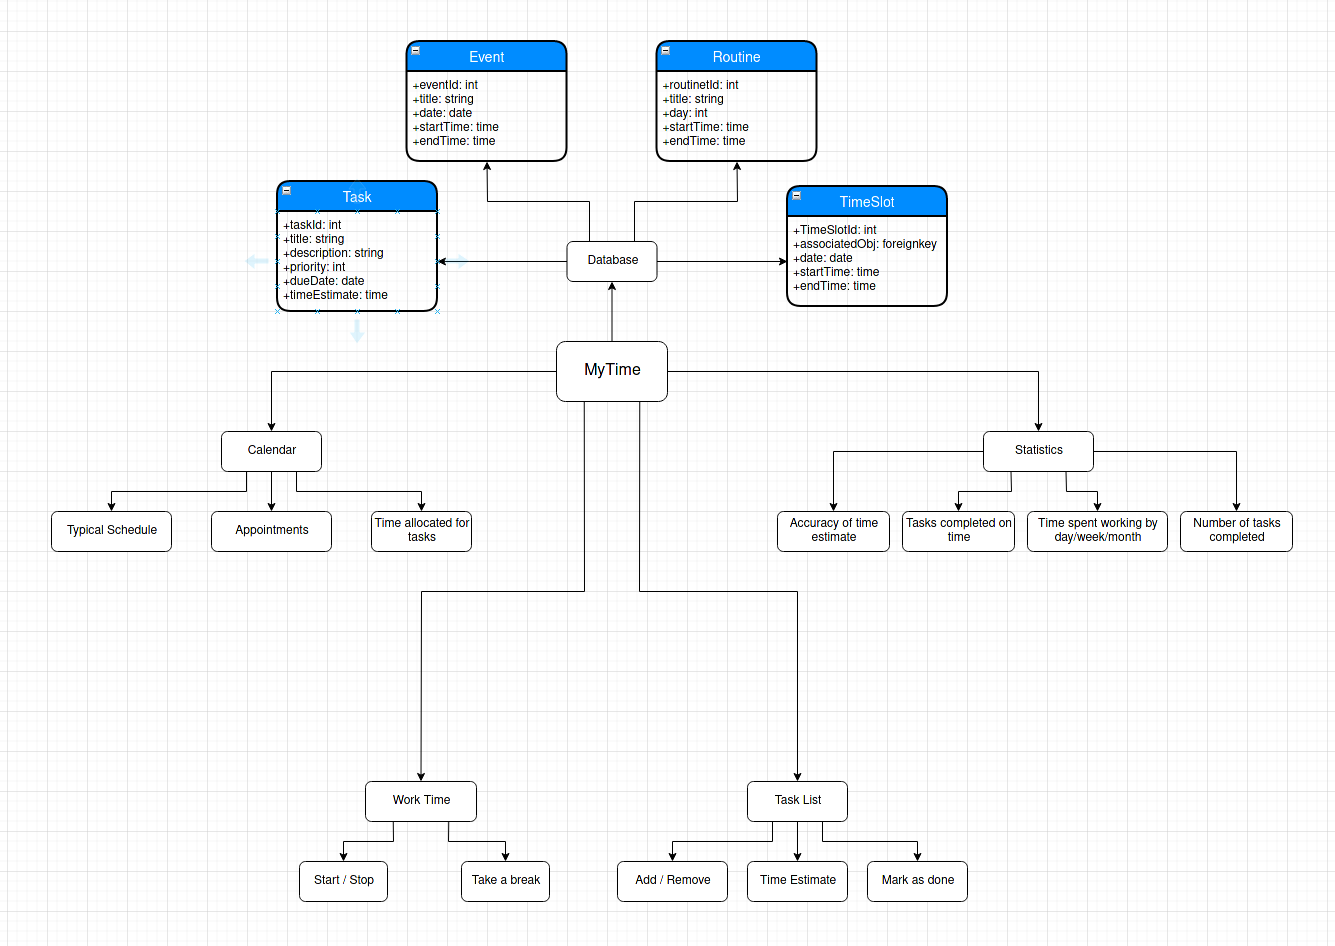
\includegraphics[width=\linewidth]{Images/TDD.png}
	\caption{Combination of top-down design analysis and class diagrams}
	\label{fig:TDD1}
\end{figure}

\subsection{Explanation of design}
The solution naturally breaks down into four parts:
a task manager,
a basic calendar,
a tracker for time spent working,
and a statistics overview.
The relevant data that each component will need to use is also quite obvious:
the task manager, time tracker and statistics tracker will only be concerned with tasks,
whereas the calendar will additionally need the user's routine, daily commitments,
and any particular events that tasks will need to be scheduled around.

The data, then, will consist of four types.
Tasks will have a title and description,
so the user can record a reasonable amount of information alongside them,
and a due date, time estimate and priority level,
so that they can be scheduled.
Events and routines are similar,
however differ in that whereas events have a concrete date,
routines have a weekday on which they reoccur.
Both have a title, start and end time.
The TimeSlot exists for the purposes of unifying data into a single type for the purposes of scheduling.
They have a date, start and end time as expected,
and additionally an associated object,
being the task, event or routine which occupies that slice of time.
It might be possible to remove the need for this additional data structure,
by instead converting tasks and routines into events for the purpose of scheduling,
however it makes sense to logically distinguish between tasks, events and routines,
which represent user intentions -
what the user wants to do with their time -
and time slots,
which represent a concrete allocation of time to be used for a specific purpose.
Of course events and routines are already concrete,
as the program will never override them since this would not be helpful for the user,
but it is a nice logical separation to make in the database,
which wouldn't be possible if I instead used the approach of converting everything into events for scheduling.
Furthermore it would bloat event records with fields that would often go unused,
depending on whether it was a regular event or a wrapper around a task or routine,
so it seems more elegant to have a separate class for time slots.

\section{UI Design}
In Django,
each page on the site is called a ``view''.
I will have the following views:
\begin{samepage}
	\begin{itemize}
		\item Task list:\\
		      A screen where the user can create, view and manage their tasks
		\item Calendar:\\
		      A screen where the user can create, view and manage upcoming events
		\item Schedule:\\
		      A screen showing the users tasks scheduled in around their events for today
		\item Task/event/routine detail:\\
		      A screen where the user can look at and individual task, event or routine,
		      and perform relevant actions such as marking as done/todo,
		      editing or deleting them
		\item Task/event/routine creator:\\
		      A form to create new tasks, events or routines
		\item Task/event/routine editor:\\
		      A form to edit existing tasks, events or routines
		\item Work time:\\
		      A screen where the user can enter a ``work session'' which records the time they spend working
		\item Work review:\\
		      A screen displaying statistics about the time the user has spent working
	\end{itemize}
\end{samepage}

I think it will also be helpful to have a navigation bar,
at the top of the screen,
allowing the user to quickly jump between the five main views -
task list, calendar, schedule, work time and work review -
and have individual tasks and events accessible from those views.
It might also be helpful to have a quick button to add a new task/event/routine.

\subsection{View Mockups}
\begin{minipage}{0.5\textwidth}
	\begin{figure}[H]
		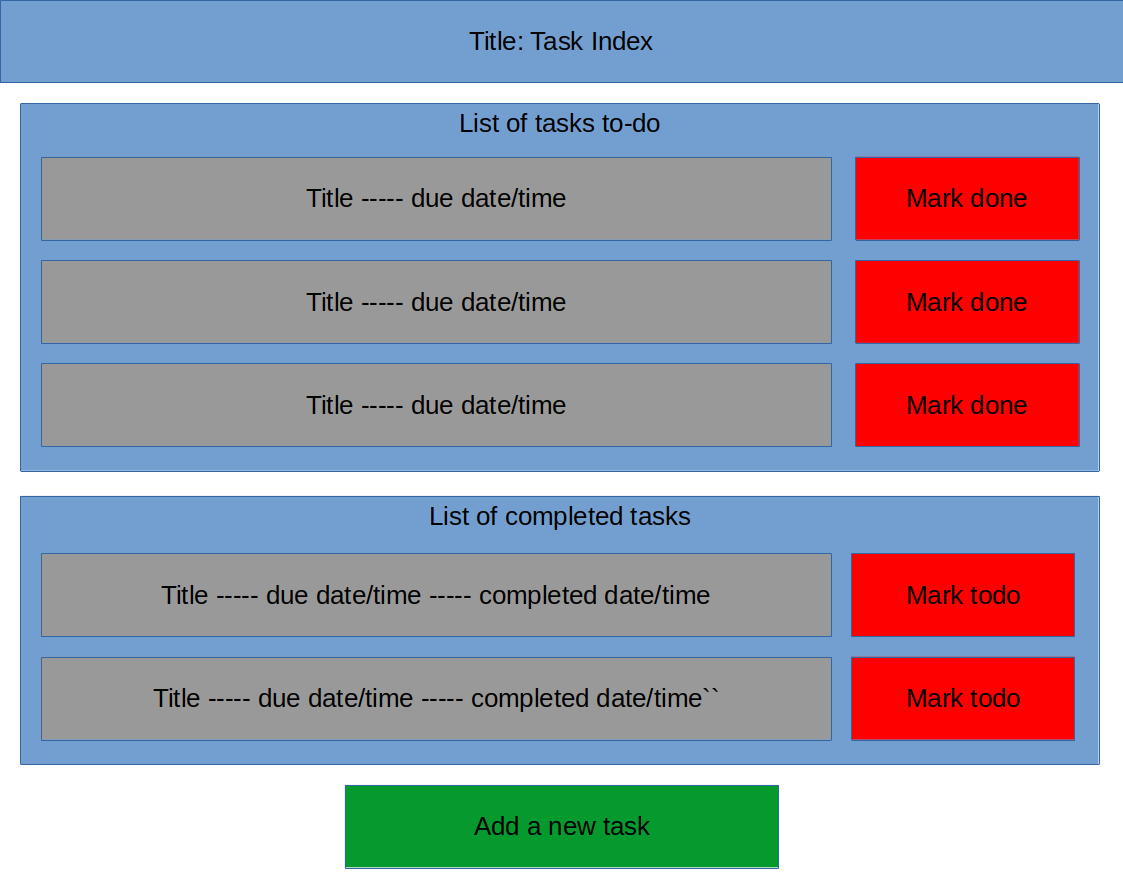
\includegraphics[width=\linewidth]{Mockups/task_index.png}
		\label{fig:task_index_mockup}
		\caption{Mockup of the task index page}
	\end{figure}
\end{minipage} \hfill
\begin{minipage}{0.45\textwidth}
	\paragraph{Features:}
	\begin{samepage}
		\begin{itemize}
			\item View all tasks
			\item List split by todo/done status
			\item Click on a task to see a more detailed view
			\item Quickly toggle whether a task is done
			\item Add new tasks
		\end{itemize}
	\end{samepage}
\end{minipage}

\begin{minipage}{0.45\textwidth}
	\begin{figure}[H]
		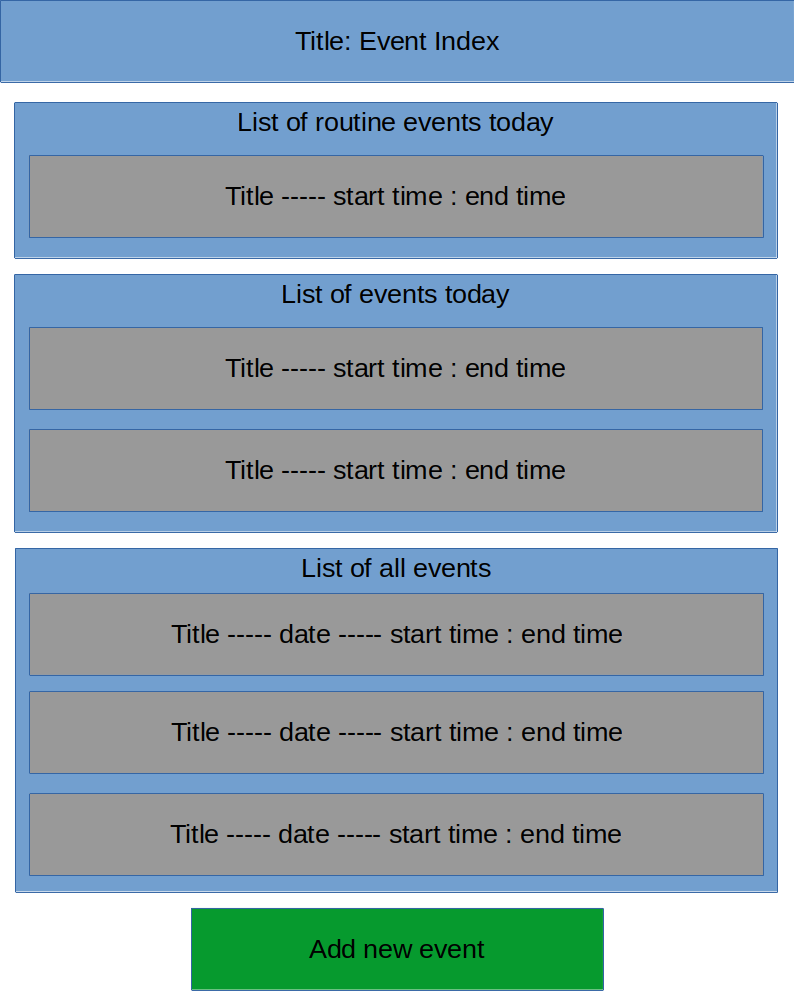
\includegraphics[width=\linewidth]{Mockups/event_index.png}
		\label{fig:event_index_mockup}
		\caption{Mockup of the calendar page}
	\end{figure}
\end{minipage} \hfill
\begin{minipage}{0.5\textwidth}
	\paragraph{Features:}
	\begin{samepage}
		\begin{itemize}
			\item View all upcoming events
			\item List split by one-off events and routine events,
			      and further by those which are today and which are later
			\item Click on and event to see a more detailed view
			\item Add new events
		\end{itemize}
	\end{samepage}
\end{minipage}

\begin{minipage}{0.5\textwidth}
	\begin{figure}[H]
		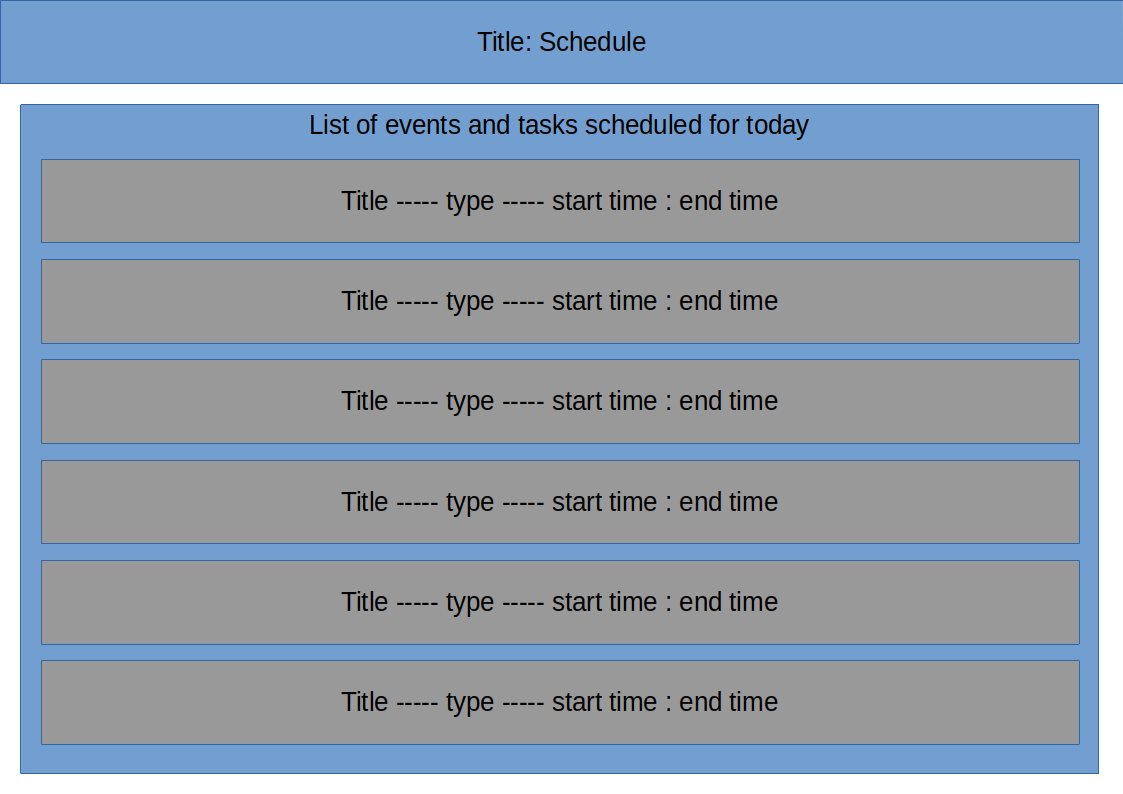
\includegraphics[width=\linewidth]{Mockups/schedule.png}
		\label{fig:schedule_mockup}
		\caption{Mockup of the schedule page}
	\end{figure}
\end{minipage} \hfill
\begin{minipage}{0.45\textwidth}
	\paragraph{Features:}
	\begin{samepage}
		\begin{itemize}
			\item View routine, events and tasks scheduled for today
			\item Tasks are scheduled automatically according to due date, priority and time estimate
			\item Click on an item to see a more detailed view
		\end{itemize}
	\end{samepage}
\end{minipage}

\begin{minipage}{0.5\textwidth}
	\begin{figure}[H]
		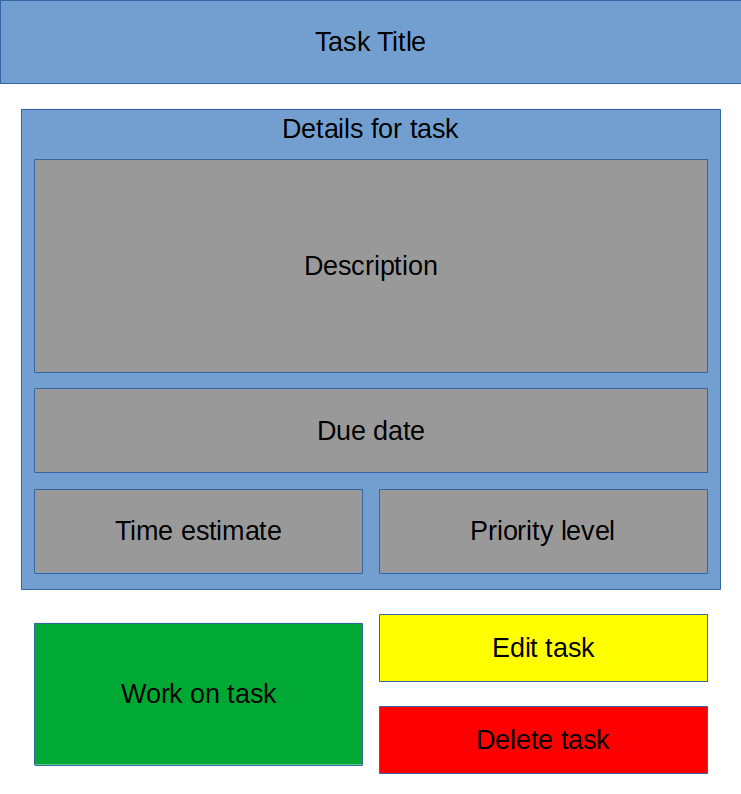
\includegraphics[width=\linewidth]{Mockups/task_detail.png}
		\label{fig:task_detail_mockup}
		\caption{Mockup of the task detail page}
	\end{figure}
\end{minipage} \hfill
\begin{minipage}{0.45\textwidth}
	\paragraph{Features:}
	\begin{samepage}
		\begin{itemize}
			\item View all the information about the task
			\item Mark the task as done/todo
			\item Edit information about the task
			\item Delete the task
			\item Log time working on the task
		\end{itemize}
	\end{samepage}
\end{minipage}

\begin{minipage}{0.5\textwidth}
	\begin{figure}[H]
		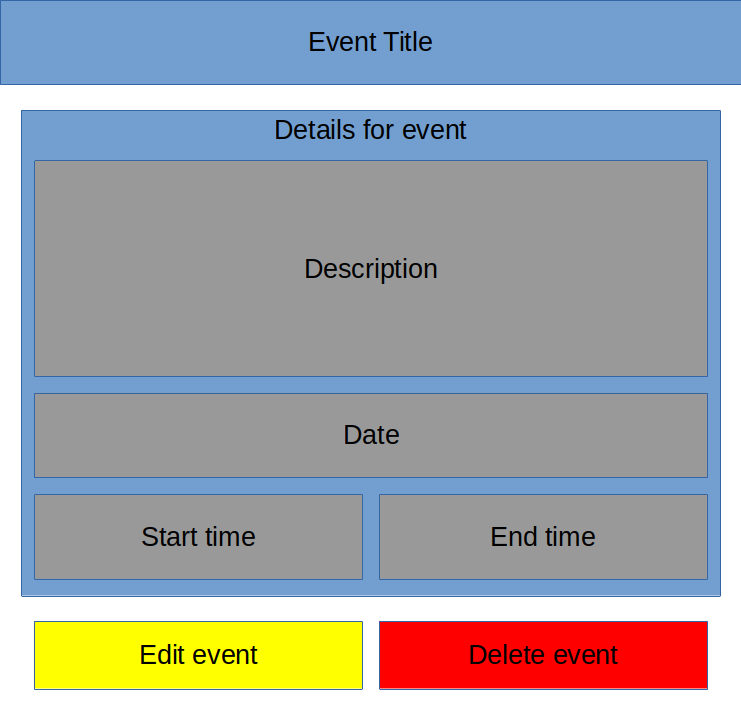
\includegraphics[width=\linewidth]{Mockups/event_detail.png}
		\label{fig:event_detail_mockup}
		\caption{Mockup of the task detail page}
	\end{figure}
\end{minipage} \hfill
\begin{minipage}{0.45\textwidth}
	\paragraph{Features:}
	\begin{samepage}
		\begin{itemize}
			\item View all the information about the event
			\item Edit information about the event
			\item Delete the event
		\end{itemize}
	\end{samepage}
\end{minipage}

\begin{minipage}{0.5\textwidth}
	\begin{figure}[H]
		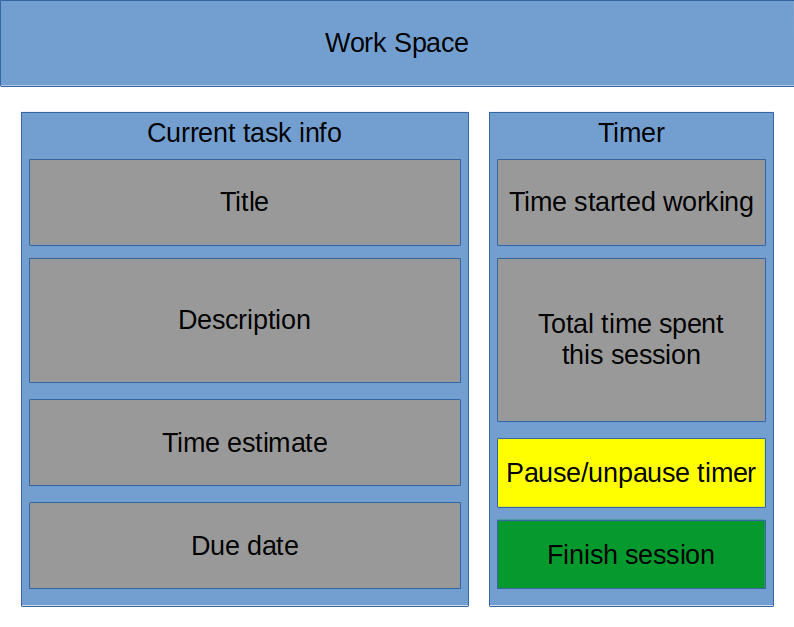
\includegraphics[width=\linewidth]{Mockups/study_space.png}
		\label{fig:work_space_mockup}
		\caption{Mockup of the work space page}
	\end{figure}
\end{minipage} \hfill
\begin{minipage}{0.45\textwidth}
	\paragraph{Features:}
	\begin{samepage}
		\begin{itemize}
			\item View information about the current task
			\item A timer of time spent working
			\item See time when started working
			\item Pause and resume the timer
			\item End the work session
		\end{itemize}
	\end{samepage}
\end{minipage}

\begin{minipage}{0.5\textwidth}
	\begin{figure}[H]
		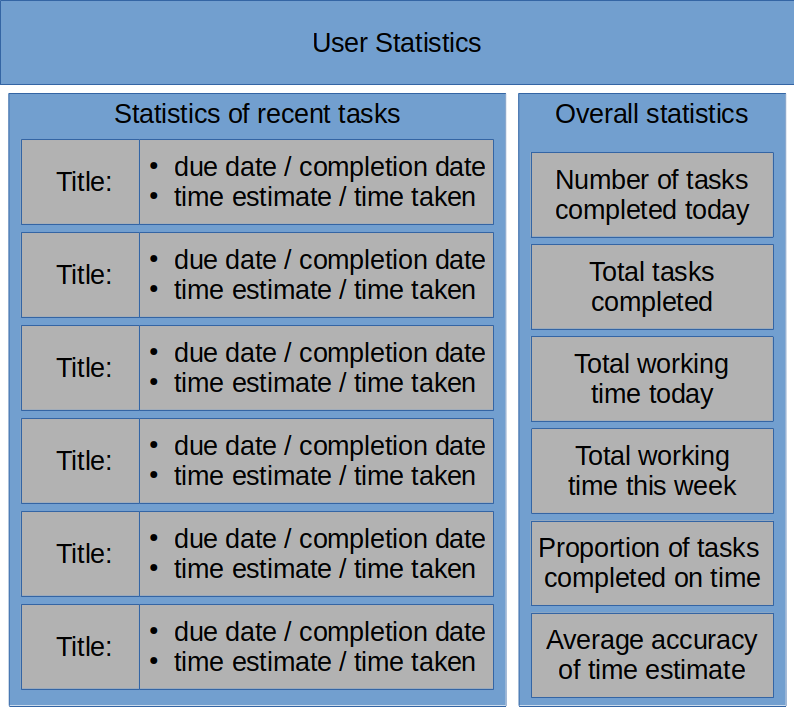
\includegraphics[width=\linewidth]{Mockups/statistics.png}
		\label{fig:statistics_mockup}
		\caption{Mockup of the work space page}
	\end{figure}
\end{minipage} \hfill
\begin{minipage}{0.45\textwidth}
	\paragraph{Features:}
	\begin{samepage}
		\begin{itemize}
			\item View individual statistics for recently completed tasks
			      \begin{samepage}
				      \begin{itemize}
					      \item Comparison of due date with date of completion
					      \item Comparison of time estimate with actual time spent
				      \end{itemize}
			      \end{samepage}
			\item View overall statistics
			      \begin{samepage}
				      \begin{itemize}
					      \item Number of tasks completed today and this week
					      \item Time spent working today and this week
					      \item Proportion of tasks completed on time
					      \item Overall accuracy of time estimates
				      \end{itemize}
			      \end{samepage}
		\end{itemize}
	\end{samepage}
\end{minipage}

\section{Usability features}
There are several notable usability features to be included.
Firstly, since there are a number of page which can display tasks, events and routines,
it will be ensured that wherever one of these is featured it will contain a link through to it's detail view.
This way the user can always quickly access the relevant information.
Secondly, todo/done toggles will be included on both the task index and task detail pages,
so the user can quickly alter any task's status.
Thirdly, there will be a navigation bar present on all pages,
so that the user can move between the main views -
the task and event lists,
the schedule page,
and the statistics page.

\section{Algorithms}
Django takes a primarily object oriented approach to creating webapps.
This means that in reality my code will consist of classes,
which describe the data and how it is laid out on the screen.
However here I will describe parts of the solution in terms of pseudocode algorithms,
where appropriate.

\subsection{Create task}
\begin{lstlisting}[breaklines]
// Get the information for the task
str title <- input(''Enter title for task'')
str description <- input(''Enter description for task'')
date due_date <- input(''Enter due date for task'')
timedelta time_estimate <- input(''Enter time estimate for task'')
int priority <- input(''Enter priority level for task'')

// Instantiate a new task object
task <- new Task

// Set the attributes according to the user input
task.set_title(title)
task.set_description(description)
task.set_due_date(due_date)
task.set_start_time(start_time)
task.set_end_time(end_time)
task.set_priority(priority)

// Save the task to the database
task.save()
\end{lstlisting}

The process for creating events and routines is largely identical.

\subsection{Update task}
\begin{lstlisting}[breaklines]
// Get input for what data needs updating
char user_input <- input(''Update information (u), change status (s), or record time spent working (t)?'')

// If the user wants to update information...
if user_input = 'u'
    // Get the new information for the task
    str new_title <- input(''Enter title for task'')
    str new_description <- input(''Enter description for task'')
    date new_due_date <- input(''Enter due date for task'')
    timedelta new_time_estimate <- input(''Enter time estimate for task'')
    int new_priority <- input(''Enter priority level for task'')

    // Update the task attributes
    task.set_title(title)
    task.set_description(description)
    task.set_due_date(due_date)
    task.set_start_time(start_time)
    task.set_end_time(end_time)
    task.set_priority(priority)
    task.save()

// If the user wants to change status...
elif user_input = 's'
    // Change the task's done status
    if task.is_done
        task.set_is_done(false)
    else
        task.set_is_done(true)
    end
    task.save()

// If the user wants to record time spent working...
elif user_input = 't'
    time t <- input(''Enter time spent'')
    task.time_spent <- task.time_spent + t
    task.save()

// Otherwise, the input was invalid
else
    print("That wasn't a valid input, please try again.")
end
\end{lstlisting}

The process for updating events and routines is similar,
however it is only possible to update the information,
as there is no status or time spent attribute.

\subsection{Make schedule}
\begin{lstlisting}[breaklines]
// Create time slots for all events and routines
for event in events where event.date = date
    ts <- new TimeSlot
    ts.set_date(date)
    ts.set_start_time(event.start_time)
    ts.set_end_time(event.end_time)
    ts.set_associated_event(event)
    ts.save()
end

for routine in routines where routine.day = date.weekday()
    ts <- new TimeSlot
    ts.set_date(date)
    ts.set_start_time(routine.start_time)
    ts.set_end_time(routine.end_time)
    ts.set_associated_routine(routine)
    ts.save()
end

// Create time slots for tasks according to free time
ts_list <- timeslots.sort_by(start_time)
for 0 <= i < len(ts_list) - 1
    // Room for change in terms of which tasks will be scheduled,
    // for example I might decide to restrict it to tasks with a due date within a certain range
    for task in tasks.sort_by(due_date, priority)
        // Again room for change in terms of how much time to leave between tasks and events,
        // I might allow the user to configure this
        if timedelta(from=ts_list[i].end_time, to=ts_list[i+1].start_time) - task.time_estimate > timedelta(minutes=10)
            ts <- new TimeSlot
            ts.set_date(date)
            ts.set_start_time(ts[i].end_time+timedelta(minutes=5))
            ts.set_end_time(ts.start_time+task.time_estimate)
            ts.set_associated_task(task)
            ts.save()
        end
    end
end
\end{lstlisting}

\subsection{Generate statistics}
\begin{lstlisting}[breaklines]
// Calculate and print statistics for recent tasks
for task in tasks where task.completed = true and task.completion_date > datetime.today() - timedelta(days=5)
    print(task.title)
    // Calculate the time delta between completion and due
    completion_time_delta <- timedelta(from=task.completion_date, to=task.due_date) + timedelta(from=task.completion_time, to=task.due_time)
    // If it was completed on time, the time delta is positive. Print it
    // NB that all tasks are flagged as completed on time or not when they are marked as done
    if task.was_completed_on_time
        print("Task was completed on time by", completion_time_delta)
    // If it was completed late, the time delta is negative, so correct that when printing
    else
        print("Task was completed late by", -1*completion_time_delta)
    end
    // Calculate the accuracy of the time estimate
    accuracy <- (task.time_estimate / task.time_spent) - 1
    // If this is positive, the user overestimated
    if accuracy > 0
        print("Overestimated time needed by", accuracy*100, "percent")
    // If it's negative, the user underestimated
    elif accuracy < 0
        print("Underestimated time needed by", accuracy*100, "percent")
    // If it's exactly 0, the estimate was perfect
    else
        print("Time estimate was perfect")
    end
end

// Calculate and print aggregate statistics
// Get a list of tasks completed today
tasks_today <- [task for task in tasks where task.completed = true and task.completion_date = datetime.today()]
print("Number of tasks completed today:", len(tasks_today)

// Sum the time spent working today
time_today <- sum([task.time_spent for task in tasks_today])
print("Time spent working today:", time_today)

// Get a list of task completed this week
tasks_week <- [task for task in tasks where task.completed = true and task.completion_date > datetime.today() - timedelta(days=7)]

// Sum the time spent working this week
time_week <- sum([task.time_spent for task in tasks_week])
print("Time spent working this week:", time_week)

// Get a list of all tasks completed
tasks_complete <- [task for task in tasks where task.completed = true]

// Calculate and print proportion of tasks completed on time
tasks_complete_on_time <- [task for task in tasks_complete where task.was_completed_on_time = true]
on_time <- len(tasks_complete_on_time) / len(task_complete)
print("Proportion of task completed on time:", on_time*100, "percent")

// Calculate and print average accuracy of time estimate
average_accuracy <- sum([(task.time_estimate / task.time_spent) - 1 for task in tasks_complete]) / len(tasks_complete
if average_accuracy > 0
    print("Average accuracy of time estimate: too great by", average_accuracy*100, "percent")
elif average_accuracy < 0
    print("Average accuracy of time estimate: too low by", average_accuracy*100, "percent")
else
    print("On average, time estimate accuracy is perfect.")
end
\end{lstlisting}

\subsection{Other parts of the solution}
This covers the dynamic aspects of the project.
Although, as discussed, there are other parts,
these aren't really possible to describe algorithmically,
since pages such as the detail views and calendar and task views are primarily static.

\section{Relations of the modules}
The top-down design breaks down the project to some extent,
however I will now outline the structure more explicitly,
and in the context of the terminology used by Django.

\begin{figure}[H]
	\centering
	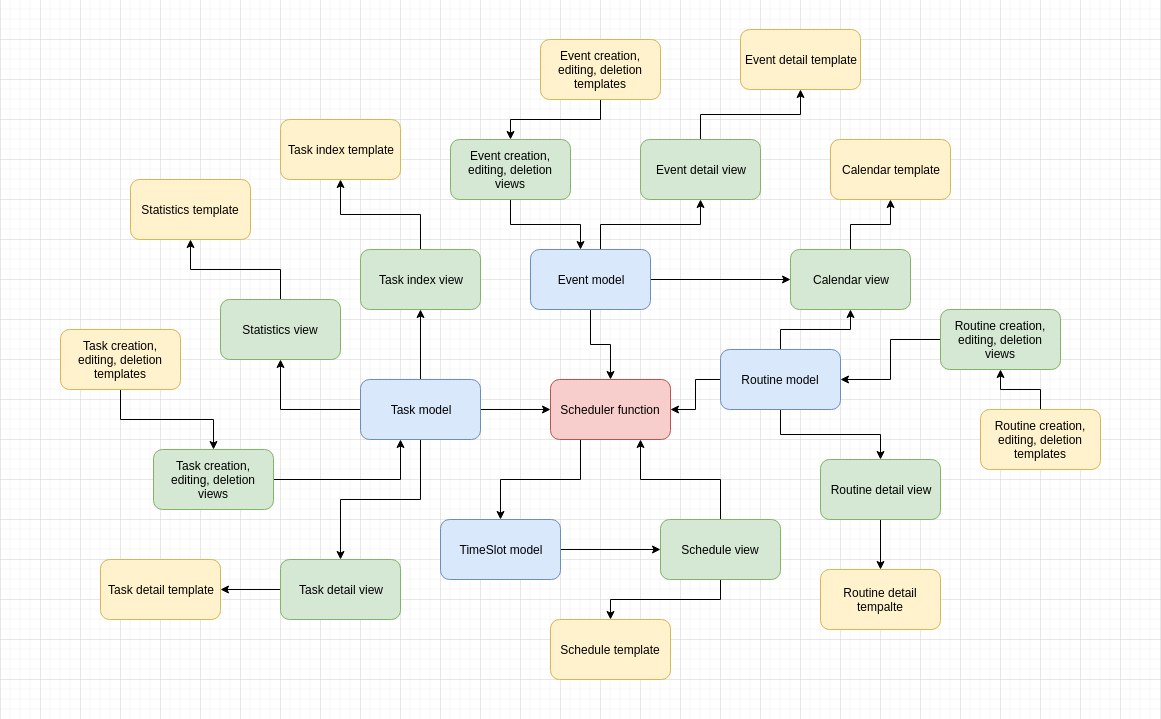
\includegraphics[width=\linewidth]{Screenshots/mytime_modular_design.png}
	\caption{Diagram of the modules showing the flow of data}
	\label{fig:modular_design}
\end{figure}

The modules have been colour coded into:
\begin{samepage}
	\begin{itemize}
		\item Red: distinct functions
		\item Blue: database models
		\item Green: page views
		\item Yellow: page templates
	\end{itemize}
\end{samepage}

This diagram shows the solution broken down into almost as small components as possible.
Note that creation, editing and deletion views for each model have been grouped together,
even though they could be distinguished,
because in terms of the flow of data,
and in the operation of the project they are obviously interdependent.
The arrows show the ``flow'' of the data,
I'll explain this with some illustrations:
new tasks are created by filling in forms in the HTML template for task creation,
which returns this data to the task view,
which creates a corresponding task model in the database;
the schedule view call the schedule function,
which takes task, event and routine models,
and creates corresponding time slot models,
which the schedule view provides the schedule template,
to render in HTML.

\part{Development}
\section{Stage 0: Learning Django}
I haven't used Django before,
so before I really get started on building my project I need to learn the basics.
Fortunately, Django have a very helpful and comprehensive tutorial,
as well as detailed and easy to navigate documentation.

I decided first of all to run through the standard tutorial,
which involves building a website for hosting various polls.
In fact, this turned out to be incredibly useful because the structure of this website bears a number of similarities to my project:
the main screen is a list of various polls,
which you can then click on to view more information about and interact with.
I will similarly need to have screens with lists of tasks and events,
which you can then view in more detail and edit or mark as done etc.

\subsection{Models and Views}
I understand that Django is oriented around two primary data structures:
models and views.
Models are classes in Python,
but they are also the tables in the database,
with the attributes of the class corresponding to the fields,
and instances to specific records.
Being objects, they can also have methods.
These don't correspond to anything in the database,
but are useful for manipulating data.
I imagine, for example, that I will want my Task model to have a mark as done method when I come to implement it.

Views, on the other hand, correspond to the frontend.
They outline what data will be viewed on each page,
and also vaguely specify the appearance of the page,
although this is controlled more precisely in HTML ``templates''.

Here is an example model from the polls tutorial:
\begin{lstlisting}[language=Python]
class Question(models.Model):
    question_text = models.CharField(max_length=200)
    pub_date = models.DateTimeField('date published')

    def __str__(self):
        return self.question_text

    def was_published_recently(self):
        return self.pub_date >= timezone.now() - datetime.timedelta(days=1)
\end{lstlisting}

In the database,
this corresponds to a table called ``Question'',
with fields ``question\_text'' and ``pub\_date'',
holding text and datetimes respectively.

Here's a screenshot of the that table:

\begin{figure}[h]
	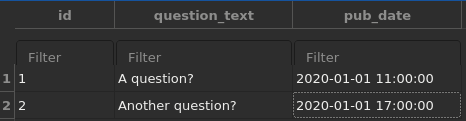
\includegraphics[width=\linewidth]{Images/question_table.png}
	\caption{Database table ``Question''}
	\label{fig:database1}
\end{figure}

As you can see,
Django also automatically includes a primary key ``id'' field with each table.

The model also has the methods ``\_\_str\_\_'' and ``was\_published\_recently'',
which are not seen in the database,
but rather make it quicker and easier to use the data within Python.

Here is an example view from the polls tutorial:
\begin{lstlisting}[language=Python]
class IndexView(generic.ListView):
    template_name = 'polls/index.html'
    context_object_name = 'latest_question_list'

    def get_queryset(self):
        # Return the last five published questions.
        return Question.objects.order_by('-pub_date')[:5]
\end{lstlisting}

The queryset for this view is the five most recently published objects in the Question table.
It then uses the template located at ``templates/polls/index.html'' -
the root folder ``templates'' is implicit.
Here is that template:
\begin{lstlisting}[language=HTML]

   <ul>
       
       <li><a href="/polls/{{ question.id }}/">{{ question.question_text }}</a></li>
       
   </ul>

   <p>No polls are available.</p>

\end{lstlisting}

Unless ``latest\_question\_list'' is empty,
this will output a list of the five most recent questions,
showing their names and linking to that question's page.
The URLs are defined in \texttt{urls.py}.

\section{Validation and Testing}
Django also provides some help with validation and testing.
Due to the connection typically present between views and models,
as long as you tell Django which forms and fields are corresponding to which models and attributes,
it will automatically validate input at both the front and backend.
For example, if a model attribute is supposed to be number between 0-5,
then Django will validate the HTML input field to require a number,
and will also make sure before submitting the data into the database that the input is between 0 and 5.
This means for the most part I won't need to manually validate input;
if I do use my own validation, I'll point that out,
otherwise it should be assumed that Django's automatic validation is being used.

With regards to testing,
Django recommends that various test be written in the \texttt{tests.py} file.
These tests can then all be run in one go,
and Django will flag any tests which failed.
The way these tests work is that a test database is created,
and one can instantiate models with various attributes,
run various methods on them,
and check that the resulting state is as expected.

\section{Stage 1: Tasks}
Given the foundations laid by my work on the tutorial,
I think the best place to start development will be with task management,
especially given that this is the primary important function of my product.

I need to make:
\begin{samepage}
	\begin{itemize}
		\item A task model,
		      to store that data about each task
		\item A task index,
		      listing todo and done tasks separately,
		      and linking through to view each task in more detail
		\item A task detail view,
		      showing all the information about a given task and allowing editing/deletion
		\item A form for adding and editing tasks
		\item A task deletion view
	\end{itemize}
\end{samepage}

\subsection{Task Model}
Logically, it makes sense to create the model first,
as we can't even begin to think about how we will display a task until we know their attributes.
Since I've already outlined the attributes and methods for it in my design,
creating the model will be quite simple.

Prototype task model:
\begin{lstlisting}[language=Python]
class Task(models.Model):
    LOW = 1
    MED = 2
    HIGH = 3
    PRIORITY_LIST = [
        (LOW, "Low"),
        (MED, "Normal"),
        (HIGH, "High"),
    ]
    title = models.CharField(max_length=200)
    description = models.CharField(max_length=1000)
    due_date = models.DateField("due date")
    due_time = models.TimeField("due time", default="23:59")
    time_estimate = models.DurationField("time estimate")
    priority = models.IntegerField("priority", choices=PRIORITY_LIST, default=2)
    done = models.BooleanField(default=False)

    def __str__(self):
        return self.title

    def is_overdue(self):
        return self.due_date <= timezone.now()

    def mark_done(self):
        self.done = True

    def mark_todo(self):
        self.done = False

    def get_absolute_url(self):
        return f"/task/{self.id}/"
\end{lstlisting}

Some notable features are the \texttt{PRIORITY\_LIST},
which is an attribute of Task but not model field -
as such it is not present in the database.
\texttt{PRIORITY\_LIST} serves the \texttt{priority} field,
which is a multiple choice field.
Choice fields require a list of tuples,
with each tuple containing a value which is actually stored in the database,
and a human readable name for that value - what it represents.
In this instance the values are \texttt{LOW}, \texttt{MED} and \texttt{HIGH},
each being a variable corresponding to the values of 1, 2 and 3 respectively,
and each with a corresponding readable name.

There is also the \texttt{get\_absolute\_url} method,
this is so it is always easy to access the corresponding detail view of any given task,
which is located at \texttt{/task/[id]}, where \texttt{id} is the task's id.
There are various ways to do this,
here I'm using an ``f-string'',
or formatted string,
so \texttt{{self.id}} will be evaluated to the id of the task.

Later in development,
I realised that the task would need some additional attributes for statistics tracking -
I could have created a separate data type for this,
but I think,
purely in terms of the code and database,
that would have been less elegant.
Additional methods and changes to the existing ones were also required to facilitate this.

\begin{lstlisting}[language=Python]
class Task(models.Model):
    # Define the choices to be used in the priority field
    LOW = 1
    MED = 2
    HIGH = 3
    PRIORITY_LIST = [
        (LOW, "Low"),
        (MED, "Normal"),
        (HIGH, "High"),
    ]
    # Define the attributes that tasks will have
    title = models.CharField(max_length=200)
    description = models.CharField(max_length=1000)
    due_date = models.DateField("due date", default=timezone.now().date())
    due_time = models.TimeField("due time", default=timezone.now().time())
    time_estimate = models.DurationField("time estimate", default=timedelta(minutes=0))
    priority = models.IntegerField("priority", choices=PRIORITY_LIST, default=2)
    done = models.BooleanField(default=False)

    # I realised later that task would additionally need these fields,
    # for the purpose of statistics tracking
    completion_time = models.DateTimeField("completion time", null=True, blank=True)
    completed_on_time = models.BooleanField(default=False)
    completed_in_time = models.BooleanField(default=False)
    time_spent = models.DurationField(
        "time spent", default=timedelta(hours=0, minutes=0)
    )
    completion_delta = models.DurationField("completion delta", null=True, blank=True)
    estimate_accuracy = models.DecimalField(
        "estimate accuracy", max_digits=4, decimal_places=1, null=True, blank=True
    )

    def __str__(self):
        return self.title

    # Check whether the task is overdue
    def is_overdue(self):
        due_datetime = datetime.combine(self.due_date, self.due_time)
        return due_datetime <= datetime.now()

    # Mark the task as done
    def mark_done(self):
        self.done = True

        # At this point we can mark whether the task was completed before it's due date,
        # and within the user's time estimate
        if self.is_overdue():
            self.completed_on_time = False
        else:
            self.completed_on_time = True
        self.completion_time = timezone.now()

        if self.time_spent <= self.time_estimate:
            self.completed_in_time = True
        else:
            self.completed_in_time = False

    # Unmark the task as done
    def mark_todo(self):
        self.done = False
        # These values need to be reset
        self.completed_on_time = False
        self.completed_in_time = False
        self.completion_time = None

    # Alter the time spent on the task
    def alter_time_spent(self, delta):
        # Time spent can't be negative, so need to check
        if (self.time_spent + delta).total_seconds() >= 0:
            self.time_spent += delta
        # If the value would be negative, just set it to 0 minutes
        else:
            self.time_spent = timedelta(minutes=0)

    def get_absolute_url(self):
        return f"/task/{self.id}/"
\end{lstlisting}

The additional attributes:
\begin{samepage}
	\begin{itemize}
		\item \texttt{completion\_time},
		      a datetime for when the task was marked as completed
		\item \texttt{completed\_on\_time},
		      a boolean for whether was or wasn't overdue at time of completion
		\item \texttt{completed\_in\_time},
		      a boolean for whether the time spent was greater or less than the time estimate at time of completion
		\item \texttt{time\_spent},
		      a timedelta for time spent working on the task
		\item \texttt{completion\_delta},
		      a time delta from completion time to due time
		\item \texttt{estimate\_accuracy},
		      the percentage (to 1 d.p.) error from the estimate to actual time taken
	\end{itemize}
\end{samepage}

These attributes are elaborated on in the Statistics and Time Tracking section of the development.

The changes to the methods,
and new method \texttt{alter\_time\_spent},
are clearly to facilitate these new attributes,
and ensure their values are always reasonable.
\texttt{mark\_done} now sets them when the task is marked as done,
and \texttt{mark\_todo} resets them.
\texttt{alter\_time\_spent} is needed for validation purposes,
to ensure that \texttt{time\_spent} does not take a negative value:
in the event the user tries to alter the time spent in a way that would make it negative,
it is simply set to 0 instead.

\subsection{Task Index}
This will consist of two parts:
a view defining the data to be displayed,
and an HTML template defining the layout.

\begin{lstlisting}[language=Python]
class IndexView(ListView):
    # Locate the HTML template
    template_name = "tasks/index.html"
    # Name the data for use in the template
    context_object_name = "task_list"

    def get_queryset(self):
        # Get all the tasks
        return Task.objects.order_by("due_date")

    def get_context_data(self, **kwargs):
        context = super(IndexView, self).get_context_data(**kwargs)
        # Get the done and todo tasks separately
        context["todo_tasks"] = Task.objects.filter(done=False).order_by("due_date")
        context["done_tasks"] = Task.objects.filter(done=True).order_by("due_date")
        return context
\end{lstlisting}

\texttt{IndexView} is a subclass of \texttt{ListView},
meaning it expects a list as its queryset -
in other words,
it retrieves a list of objects from the database,
not just one.
Therefore the \texttt{get\_queryset} returns a list of all the Task objects,
ordered by when the are due.
This data will be referred to as ``task\_list'' in the HTML template,
as specified by the \texttt{context\_object\_name} attribute.

The \texttt{get\_context\_data} function serves to segregate the data:
I split it into the tasks which are todo and which are done,
so it will be easy to show them in two separate lists.

The HTML template is specified at \texttt{templates/tasks/task\_detail.html}
(as a relative path from \texttt{models.py}),
as indicated by the attribute \texttt{template\_name}.
Having the \texttt{tasks/} subfolder is somewhat redundant,
this is just following Django's recommended directory layout,
which would help if I ever expanded the project to need more complex namespacing.
The template for this view is somewhat lengthy,
so I won't put it all here;
in short,
It will show two lists,
one of tasks which are todo,
and one of tasks which are already done.
Each task will show it's name,
doubling as a link to the detail view of the task.
It will also have a button to quickly toggle the tasks todo/done status.

Here is a snippet of that part of the code:
\begin{lstlisting}[language=HTML]
<li><a href="/task/{{ task.id }}/">{{ task.title }}</a>
    
    <form action="" method="post">
        
        <input type="hidden" name="link" value="{{ request.path }}">
        <input type="submit", value="Mark as todo">
    </form>
    
    <form action="" method="post">
        
        <input type="hidden" name="link" value="{{ request.path }}">
        <input type="submit", value="Mark as done">
    </form>
    
</li>
\end{lstlisting}

Most of this is fairly standard:
a list item,
with a hyperlink displaying the title of the task and linking to it's detail view,
and a form with a button to either mark as todo or done depending on the task's status.
Of note however are the dynamic functionalities provided by Django:
variables provded from the queryset are surrounded by double braces,
which Django replaces with the actual values when the page is visited,
and this is used for the \texttt{task.id} and \texttt{task.title} here.
Conditionals and loops are also available,
I've used an if/else statement here and,
this snippet is actually inside a for-loop,
so it creates list items for all the tasks.

The form has a \texttt{csrf\_token}:
CSRF here stands for cross-site request forgery.
Although security is far from a huge concern in my project,
Django requires this to be used by all forms.
and is certainly a best practice.
Finally, note that the URL for the form is not a hard link,
but instead makes use of the namespacing provided by Django.
\texttt{mark\_as\_done} and \texttt{mark\_as\_todo} are specified in my urls.py file,
as linking to views of the same name,
which run the relevant code to the mark the task as done or todo.
This is just one line of course,
calling the relevant method on the Task object provided by the form.
Figure \ref{fig:task_index1} shows what we've made so far.

\begin{figure}[H]
	\centering
	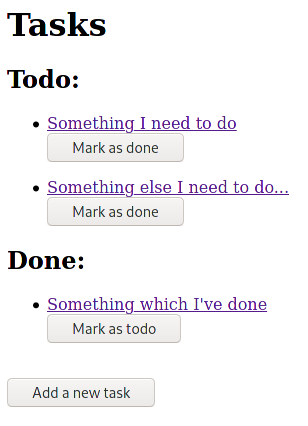
\includegraphics[width=0.5\linewidth]{Screenshots/task_index.png}
	\caption{The task index}
	\label{fig:task_index1}
\end{figure}

\subsection{Task Detail}
Currently,
the hyperlinks on the index page produce a 404 error,
because I haven't actually created the detail view for the tasks yet.
It's fairly simple,
it just needs to show the user all the information about a specific task.

Prototype task detail view:
\begin{lstlisting}[language=Python]
class TaskDetail(DetailView):
    model = Task
    template_name = "tasks/task_detail.html"

    def task_done(self):
        Task.mark_done()

    def task_todo(self):
        Task.mark_todo()
\end{lstlisting}

\texttt{TaskDetail} is a subclass of \texttt{DetailView}.
With the model specified as \texttt{Task},
this means that whenever the relevant URL is accessed,
which I've specified \texttt{tasks/[task id]},
it will get the data for the task of that id.
It also has two simple methods to be able to mark the task as todo or done.

The HTML template is also simple,
just displaying the data about the task along with a button to either mark as todo or done,
as appropriate,
a button to edit the task,
and a button to delete the task.
The latter two are not yet functional,
of course.

\begin{figure}[H]
	\centering
	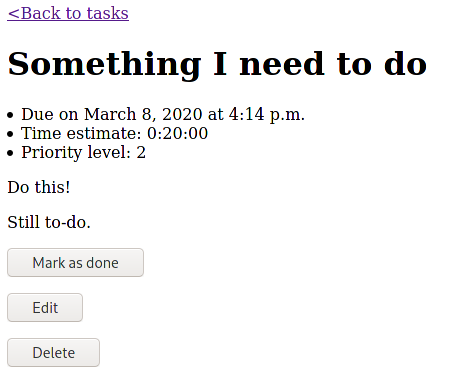
\includegraphics[width=0.6\linewidth]{Screenshots/task_detail.png}
	\caption{Detail view of a task}
	\label{fig:task_detail1}
\end{figure}

Later in development,
I made the decision to have time tracking done from the task detail page;
this is explained in detail in the Statistics and Time Tracking section.

\begin{lstlisting}
class TaskDetail(DetailView):
    model = Task
    template_name = "tasks/task_detail.html"

    # Provide a method to mark the task as done
    def task_done(self):
        Task.mark_done()

    # Provide a method to mark the task as todo
    def task_todo(self):
        Task.mark_todo()

    # Provide a method to alter the time
    def task_time_alter(self, mins):
        # Convert the inputted integer to a timedelta of that many minutes
        time_delta = timedelta(minute=mins)
        # Run the task time-alteration method
        Task.alter_time_spent(time_delta)
\end{lstlisting}

This simply involved the addition of the \texttt{task\_time\_alter} method,
and a corresponding form in the HTML template.

\subsection{Task creation/editing/deletion}
Django can automagically create basic forms for creating and updating model objects.
One just needs to specify what model a form is operating on,
what attributes should be available to alter,
and any specific widgets to be used for entering data for each field.
Then it will retrieve the values from the fields in the form with the matching name,
and create a new object or change an existing one to match the input.

\begin{lstlisting}[language=Python]
class TaskCreate(CreateView):
    model = Task

    # The fields the user is allowed to set when creating a task
    fields = [
        "title",
        "description",
        "due_date",
        "due_time",
        "time_estimate",
        "priority",
    ]

    # Provide specialised input for the due date and time
    due_date = forms.DateField(widget=forms.SelectDateWidget(attrs={"type": "date"}))
    due_time = forms.TimeField(widget=forms.TimeInput(attrs={"type": "time"}))
\end{lstlisting}

Django will default to using the template at \texttt{[model]\_form.html},
and I decided not to alter that,
which is why no template is specified here.
The template simply sonsits of a single form with input fields for each of the attributes.

The \texttt{TaskUpdate} view is overwhelingly similar,
with the simple addition that each field in the template has a default value,
being the current value of the relevant attribute.
See figure \ref{fig:task_form1}.

\begin{figure}[H]
	\centering
	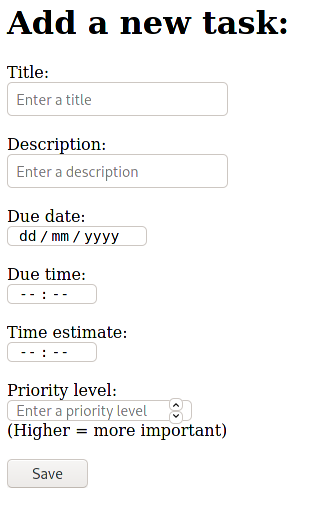
\includegraphics[width=0.5\linewidth]{Screenshots/task_form.png}
	\caption{Detail view of a task}
	\label{fig:task_form1}
\end{figure}

The deletion view is rather simple,
the only notable feature is how it redirects the user back to the index,
as going back the previous page wouldn't workm
since that would be the detail view of a task that was just deleted.

\begin{lstlisting}[language=Python]
class TaskDelete(DeleteView):
    model = Task
    # Return to the index on a successful completion
    success_url = reverse_lazy("tasks:index")
\end{lstlisting}

Likewise,
the HTML template for this view is just a form asking the user to confirm the deletion,
with a button to do so.

At this point,
it is possible to create and manage various tasks,
view them together or individually in more detail,
mark them as todo or done,
and delete them -
all the functions of a basic todo list app.
The next step is to add similar abilities for events and recurring events (routines).
This should mostly be straightforward,
as they will be in many ways like tasks,
just less dynamic,
and having a fixed start and end time.
As of yet tasks have no location in time -
they have a due date,
but no date or time specified in which they should actually be completed.
Once I've added what is essentially calendaring functionality with events and routines,
I'll write scheduler,
which will be responsible for giving tasks that anchoring in time.

\subsection{Stage 1 Testing}
The main subject for testing here is the task model.
The main way to perform tests is Django is through the use of the \texttt{TestCase} class,
which allows one to create a test database,
and use various assertion statements to check information about the database.
Here's one of the tests:
\begin{lstlisting}[language=Python]
class TaskModelTests(TestCase):
    # Test that marking a task as done works as expected
    def test_mark_done_on_todo_task(self):
        # Create a task that is todo
        todo_task = Task(done=False)
        # Get the time before
        before = timezone.now()
        # Mark task as done
        todo_task.mark_done()
        # Get the time after
        after = timezone.now()

        # Check that the task is indeed marked as done
        self.assertIs(todo_task.done, True)

        # Check that the task was completed between the two timestamps
        not_too_early = bool(todo_task.completion_time >= before)
        not_too_late = bool(todo_task.completion_time <= after)

        self.assertIs(not_too_early, True)
        self.assertIs(not_too_late, True)
\end{lstlisting}

Let me walk this through in detail.
Tests are written as methods of a class which inherits from \texttt{TestCase}.
Here I've called the class \texttt{TaskModelTests}.
The first test is one for checking the functionality of the \texttt{mark\_done} method,
on a task which is still todo.
I want to test
\begin{samepage}
	\begin{enumerate}
		\item that the task is indeed marked as done after the method is run
		\item that the completion time is assigned correctly
	\end{enumerate}
\end{samepage}
so I take time snapshots before and after marking the task as done.
Then I check that the task's \texttt{done} attribute is true,
using the assertion method provided by the \texttt{TestCase} class.
Next, I assign two variables,
\texttt{not\_too\_early} and \texttt{not\_too\_late},
respectively to whether the completion time of the task is after the \texttt{before} datetime,
and before the \texttt{after} datetime -
i.e. both these variables will be true if the completion time is between the two timestamps,
as it should be.
Finally, I assert that both these variables are true.

Here are the rest of the tests for the task model:
\begin{lstlisting}[language=Python]
    # Test that marking a task as todo works as expected
    def test_mark_todo_on_done_task(self):
        # Create a task that is done
        done_task = Task(done=True)
        # Mark it as todo
        done_task.mark_todo()

        # Check the task is not marked as done
        self.assertIs(done_task.done, False)

        # Check that the completion time has been reset
        self.assertEquals(done_task.completion_time, None)

    # Test that the overdue method works correctly
    def test_is_overdue_on_not_overdue_task(self):
        # Create a task that is not overdue
        non_overdue_task = Task(
            due_date=dt.date.today() + dt.timedelta(days=1),
            due_time=dt.time(hour=0, minute=0),
        )

        # Check that the method finds it to not be overdue
        self.assertIs(non_overdue_task.is_overdue(), False)

    def test_is_overdue_on_overdue_task(self):
        # Create a task that is overdue
        overdue_task = Task(
            due_date=dt.date.today() - dt.timedelta(days=1),
            due_time=dt.time(hour=0, minute=0),
        )

        # Check that it is found to be overdue
        self.assertIs(overdue_task.is_overdue(), True)

    # Basic test for time spent alteration
    def test_alter_time_spent(self):
        # Create a taskwith no time spent
        no_time_task = Task()

        # Increase time spent by 10 minutes
        no_time_task.alter_time_spent(dt.timedelta(minutes=10))

        # Check that the time spent is correct
        self.assertEquals(no_time_task.time_spent, dt.timedelta(minutes=10))

    # Test that when altering a task to have negative time spent,
    # it instead is set to 0
    def test_alter_time_spent_negative(self):
        # Create a task with 10 minutes time spent
        ten_minute_task = Task(time_spent=dt.timedelta(minutes=10))

        # Reduce time spent by 20 minutes
        ten_minute_task.alter_time_spent(timedelta(minutes=-20))

        # Time spent should now be 0 minutes, rather then -10
        self.assertEquals(ten_minute_task.time_spent, timedelta(minutes=0))
\end{lstlisting}

The comments here should be sufficient to make it clear what each task does.
One thing worth explaining is the use of \texttt{assertEquals},
rather than \texttt{assertIs} in some places:
this is because \texttt{assertIs} is only for boolean comparisons.

When I ran these tests I encountered one error.
In fact this wasn't a problem with any of my assert statements,
rather an error was encountered in the line \lstinline{no_time_task.alter_time_spent(dt.timedelta(minutes=10))}.
When this line was run,
the value for \texttt{time\_spent} was actually null,
so when the time alteration method tried to add the input timedelta to the existing time spent,
it encountered an error,
since you can't add \texttt{timedelta} to \texttt{None}.
I rectified this by adding a default value of a 0 minute timedelta to that attribute.
This was a good error to catch,
as it would have completely broken all time-logging functionality,
since, without the default value,
all tasks would start with a null time spent.

With regard to testing views,
Django also provides a framework for testing these,
however this is quite complicated would require,
I think,
an unreasonable amount of time to learn.
So I went ahead with testing manually.
In particular, I looked at:
\begin{samepage}
	\begin{itemize}
		\item the mark todo/done buttons on the task index and task detail pages
		\item whether the views for creating, updating and deleting tasks worked correctly
	\end{itemize}
\end{samepage}

I verified that use of the mark todo/done buttons produced corresponding change in the database,
and that the values input to the forms on the task creation and updating pages created the correct attributes in the corresponding task.
If any field contains an invalid input when the form is submitted,
the database will not be affected and the user must correct the problem.
Finally,
the task deletion view does correctly delete the corresponding task from the database.

\subsection{Stage 1 Review}
This stage was overall quite a success,
especially given that one might expect more problems to come up at the start of the project.
I think I largely attribute this taking the time to walk through Django's tutorial,
familiarising myself with the tools available,
prior to diving into development of the project proper.
Clearly the most notable issue with this stage were the omissions,
which I needed to come back and fix when I realised that they were missing.
More care in the design stage could have helped to avoid this.
However, thankfully, this turned out not to be a very big issue,
and was easily corrected.

So at the end of stage 1 it is now possible to:
\begin{samepage}
	\begin{itemize}
		\item Create tasks
		\item View the list of tasks which are still todo and which are done
		\item View a page with detailed information about each task
		\item Edit a task or delete it
		\item Toggle whether a task is todo or done,
		      from either the index or the detail pages
	\end{itemize}
\end{samepage}

In other words,
the task management component is fully functional.

\section{Stage 2: Events and Routines}
Events and routines will be like tasks in many ways.
In fact,
I considered whether it might be better to refactor my task models to be slightly more general,
then have each of events, tasks and routines inherit from it.
If all that my project consisted of was Python with ordinary classes and objects,
I might have gone this route,
however the problem is that models aren't merely classes in Python but also represent tables in the database.
Whereas it wouldn't be such a problem for classes to have unused attributes,
I'm not happy with the idea of each entry in the database having many empty fields.
Technically there is nothing specifying that this is bad practice in database design -
I don't believe any of the normal forms require that fields not be ``excessively null'',
as it were,
however I simply find the notion quite unappealing.
So I think it's the nicer solution to separate each out into it's own model.

On a similar point,
events and routines might really seem similar enough to use the same model,
however routines need to be treated differently due to their recurrence:
routines happen on a day of the week,
every week,
as opposed to events which happen once on a specified data.
I think that combining them would result in potential complexity or room for confusion,
so I decided to go with this route.

\subsection{Models}
The event model has a title, date, start and end times,
and a flag for if it should override a routine if it clashes.
It has several getters,
and additionally a method to check if it clashes with another event/routine.

\begin{lstlisting}[language=Python]
def does_clash(self, other):
    # For events A and B to clash,
    # A must start before B ends and end after B starts
    if self.start_time < other.end_time and self.end_time > other.start_time:
        return True
    else:
        return False
\end{lstlisting}

It took me a few tries to figure out how exactly to formulate that if condition.
The logic is this:
if event A starts before B ends,
and A hasn't finished by the time B starts,
then they must overlap.

The routine model is very similar,
however it has a day instead of a date,
which is a selection from Monday through Sunday.

\subsection{Views}
Events and routines each have detail, creation, updating and deletion views similar to tasks.
There is also an event and routine index similar to the task index.
Apart from the index these views aren't worthy of much discussion,
due to their similarity with the corresponding task views.

\begin{lstlisting}[language=Python]
class EventView(ListView):
    template_name = "tasks/event_index.html"
    context_object_name = "event_list"

    def get_queryset(self):
        # Get the events in order of their date
        return Event.objects.order_by("date")

    def get_context_data(self, **kwargs):
        context = super(EventView, self).get_context_data(**kwargs)
        # Get today's events in time order
        context["events_today"] = Event.objects.filter(date=datetime.today()).order_by(
            "start_time"
        )
        # Likewise for today's routine events
        context["routine_today"] = Routine.objects.filter(
            day=datetime.today().weekday()
        ).order_by("start_time")
        # Likeise for all events and routine events
        context["events"] = Event.objects.order_by("date", "start_time")
        context["routine"] = Routine.objects.order_by("day", "start_time")
        return context
\end{lstlisting}

The notable aspect here is that it is retrieving the data for both events and routines,
something which none of my views have done thus far.
It retrieves events for today,
routines for today,
all events,
and all routines,
into separate entries in the \texttt{context} dictionary,
each ordered by date/day and start time,
so each can be displayed separately in chronological order.
It makes sense to separate out the tasks and routines that are on today,
so that they can be displayed more prominently.

\subsection{Stage 2 Testing}
The models here are relatively simpler,
compared to the task model.
The only thing to test here is the \texttt{does\_clash} method of the event model.

\begin{lstlisting}[language=Python]
class EventModelTests(TestCase):
    # Test non-overlapping events
    #
    # Test events that are on the same day and nearly overlap, but don't
    def test_same_day_no_time_overlap(self):
        # Define two events which are consecutive but don't overlap
        event_1 = Event(
            date=timezone.now().date(),
            start_time=(timezone.now() - dt.timedelta(minutes=10)).time(),
            end_time=timezone.now().time(),
        )
        event_2 = Event(
            date=timezone.now().date(),
            start_time=timezone.now().time(),
            end_time=(timezone.now() + dt.timedelta(minutes=10)).time(),
        )

        # Neither should clash with the other
        self.assertIs(event_1.does_clash(event_2), False)
        self.assertIs(event_2.does_clash(event_1), False)

    # Test events where the time overlaps but are on different days
    def test_different_day_overlapping_time(self):
        # Define two events which would clash if they were on the same day,
        # but are on different days
        event_1 = Event(
            date=timezone.now().date(),
            start_time=timezone.now().time(),
            end_time=(timezone.now() + dt.timedelta(minutes=10)).time(),
        )
        event_2 = Event(
            date=(timezone.now() + dt.timedelta(days=1)).date(),
            start_time=(timezone.now() - dt.timedelta(minutes=5)).time(),
            end_time=(timezone.now() + dt.timedelta(minutes=5)).time(),
        )

        # Neither should clash with the other
        self.assertIs(event_1.does_clash(event_2), False)
        self.assertIs(event_2.does_clash(event_1), False)

    # Test overlapping events
    #
    # Test events overlapping only at one end
    def test_overlap_one_end(self):
        # Define two events which overlap only on one end
        event_1 = Event(
            date=timezone.now().date(),
            start_time=timezone.now().time(),
            end_time=(timezone.now() + dt.timedelta(minutes=10)).time(),
        )
        event_2 = Event(
            date=timezone.now().date(),
            start_time=(timezone.now() - dt.timedelta(minutes=5)).time(),
            end_time=(timezone.now() + dt.timedelta(minutes=5)).time(),
        )

        # Both should clash with the other
        self.assertIs(event_1.does_clash(event_2), True)
        self.assertIs(event_2.does_clash(event_1), True)

    # Test events overlapping at both ends
    def test_overlap_both_ends(self):
        # Define two events which overlap at both ends
        event_1 = Event(
            date=timezone.now().date(),
            start_time=timezone.now().time(),
            end_time=(timezone.now() + dt.timedelta(minutes=10)).time(),
        )
        event_2 = Event(
            date=timezone.now().date(),
            start_time=(timezone.now() - dt.timedelta(minutes=5)).time(),
            end_time=(timezone.now() + dt.timedelta(minutes=15)).time(),
        )

        # Both should clash with the other
        self.assertIs(event_1.does_clash(event_2), True)
        self.assertIs(event_2.does_clash(event_1), True)
\end{lstlisting}

As I was writing these tests I actually realised that one of them would definitely fail:
the test for events on the same time but different days.
In fact this might seem quite an odd thing to test,
but I realised that the \texttt{does\_clash} function didn't check at all whether the two events were on the same day.
As expected, that test did fail,
so I fixed the function.

Here's the corrected version:
\begin{lstlisting}[language=Python]
def does_clash(self, other):
    # For events A and B to clash,
    # A must start before B ends and end after B starts
    if (
        self.date == other.date
        and self.start_time < other.end_time
        and self.end_time > other.start_time
    ):
        return True
    else:
        return False
\end{lstlisting}

With this fix all the tests now pass.

Then I went on to test the views in a similar manner to the task related views,
however there was less to do due the less dynamic nature of events an routines.
As one might expect,
given that the task views already worked and the similarity with the event and routine views,
there were no problems here.

\subsection{Stage 2 Review}
This stage was a bit easier than stage 1,
due to the overall similarities the event- and routine-related models and views,
had with the already existing task model and related views.
This meant the ideas and principles behind that stage of development could mostly be recycled,
with changes to the code itself mostly being small changes and simplifications.
The only hitch was that error in the \texttt{does\_clash} method for events,
which was fixed easily.

So at the end of stage 2 it is now possible to:
\begin{samepage}
	\begin{itemize}
		\item Create events
		\item View them in a list,
		      separated by whether they are on today or some other day in the future
		\item View a detailed information page about them
		\item Edit or delete existing events
		\item And do all the same things for routine events
	\end{itemize}
\end{samepage}

In other words,
full calendaring functionality.

\section{Stage 3: The Scheduler}
The scheduler consists of two parts:
a view where the events and scheduled tasks can be seen together,
and a function responsible for scheduling the tasks relative to the events.
It won't make much of a difference,
but I will put the scheduler in it's own file,
\texttt{scheduler.py},
as although it will exclusively be called by the view,
it doesn't really make sense to put it in the \texttt{views.py} file.

\subsection{The Scheduling Function}
Something which I considered,
while implementing the scheduler,
is how exactly it should manage tasks, events and routines relative to each other.
Clearly, it would be easiest to convert them all into a singular data type,
so they can be operated on in the same way.
One possible approach I considered was casting routines and tasks into events,
since events have a fixed date, start and end time,
which is all the information needed for scheduling purposes.
However, this would require adding additional clutter into the event table,
as fields would be needed to flag whether it was an ordinary event,
an event converted from a routine or an event converted from task,
and a foreign key field to link to the actual task or event it was converted from.

Instead,
I decided to create a new model for the specific purpose of representing chunks of time.
\texttt{TimeSlot} is a model with a date, start and end time,
and an associated object being a task, event or routine.
It doesn't need a name/title as this can simply be retrieved from the associated object.

Prototype time slot model:
\begin{lstlisting}[language=Python]
class TimeSlot(models.Model):
    date = models.DateField("date")
    start_time = models.TimeField("start time")
    end_time = models.TimeField("end time")
    associated_object = models.ForeignKey(on_delete=models.CASCADE, null=True)

    def get_date(self):
        return self.date

    def get_start(self):
        return self.start_time

    def get_end(self):
        return self.end_time
\end{lstlisting}

Note that for the foreign key it has the argument \texttt{on\_delete=models.CASCADE}.
This ensures referential integrity as if the associated object is deleted,
the time slot will be deleted as well.

After creating the scheduler,
I then found out that it didn't work,
because I had misunderstood the way the \texttt{ForeignKey} field worked.
In fact it's not so simple as to have a foreign key which can go to a task, event or routine,
Django requires that the type of model which a foreign key field will refer to be defined.
The result of this is,
unfortunately,
possible the ugliest thing in this entire project:
the model needs to have attributes for the type of the associated object,
and attributes for an associated task, event and routine,
with two of those being null.
The alternative would have been to create three different time slot models,
each corresponding to task, event or routine,
however that would defeat the entire point of having a single data type,
to unify everything for scheduling purposes.
So I decided that I didn't really have an option but to go ahead with this workaround.

So the time slot model ended up like this:
\begin{lstlisting}[language=Python]
class TimeSlot(models.Model):
    # Define the options to be used in the associated type field
    TYPE_CHOICES = [
        ("T", "task"),
        ("E", "event"),
        ("R", "routine"),
    ]

    # Define the attributes
    date = models.DateField("date")
    start_time = models.TimeField("start time")
    end_time = models.TimeField("end time")

    # Faciltate tracking of the associated object
    associated_type = models.CharField("type", max_length=200, choices=TYPE_CHOICES)
    associated_task = models.ForeignKey(Task, on_delete=models.CASCADE, null=True)
    associated_event = models.ForeignKey(Event, on_delete=models.CASCADE, null=True)
    associated_routine = models.ForeignKey(Routine, on_delete=models.CASCADE, null=True)

    def get_date(self):
        return self.date

    def get_start(self):
        return self.start_time

    def get_end(self):
        return self.end_time

    def __str__(self):
        return f"TimeSlot type {self.associated_type}"

    def __repr__(self):
        return f"TimeSlot type {self.associated_type}"
\end{lstlisting}

As for the scheduler itself, it:
\begin{samepage}
	\begin{itemize}
		\item Gets all the events, routines and tasks from the database
		\item Creates time slots for all the events and routines
		\item Puts them into a list in order
		\item Iterates over all the tasks according to their due date, time estimate and priority level,
		      for each one finding an available space between sequential timeslots
		      where the gap it at least as large as the time estimate for the task
		\item When a space is found, creates a time slot for the task at that time
		\item Returns a list of time slots and enters them into the database
	\end{itemize}
\end{samepage}

Here is the code for the scheduler and it's supplementary functions.
I took particular care to thoroughly comment this code,
so reading it should make clear how it works:
\begin{lstlisting}[language=Python]
# We'll need to be able to figure out a concrete date to place routine events on
# by deriving it from the current date and their assigned weekday
def get_date_from_weekday(day):
    today = datetime.today()
    delta = (day - today.weekday()) % 7
    date = datetime.today() + timedelta(days=delta)
    return date


# When we run the scheduling algorithm, we'll want to clean out any time slots
# from last time
def clean_time_slots(date):
    TimeSlot.objects.filter(date=date).delete()


# Here's the scheduler, it runs based on a given weekday rather than a date.
# This makes things easier
def update_schedule(day):
    # Get the date and clean out time slots
    date = get_date_from_weekday(day)
    clean_time_slots(date)

    # Get all events and routine events for today, ordered by start time
    routines = Routine.objects.filter(day=day).order_by("start_time")
    events = Event.objects.filter(date=date).order_by("start_time")

    # Sort them together
    all_events = sorted(
        chain(routines, events), key=lambda instance: instance.start_time
    )

    # NB I decided not to check for clashes between events/routines,
    # since there isn't really anything to do in such a case -
    # I could force them to separate,
    # but this might be undesired or unexpected for the user,
    # so I decided just to trust the user and let them handle such clashed,
    # as it won't affect task scheduling because there is no gap between them.

    # Get all the tasks, ordered by due date, time estimate and descending priority level
    tasks = Task.objects.filter(done=False).order_by(
        "due_date", "time_estimate", "-priority"
    )

    # Convert the iterable into a list, this is easier to handle and we can remove tasks
    # from the list once they have been allocated a time slot
    task_list = list(tasks)

    # Initialise an empty list for holding the time slots, we'll write them all to the
    # database at the end
    time_slots = []

    # Iterate over all the events and routines,
    # creating corresponding time slots
    for item in all_events:
        if isinstance(item, Event):
            time_slots.append(
                TimeSlot(
                    date=date,
                    start_time=item.get_start(),
                    end_time=item.get_end(),
                    associated_type="E",
                    associated_event=item,
                )
            )

        elif isinstance(item, Routine):
            time_slots.append(
                TimeSlot(
                    date=date,
                    start_time=item.get_start(),
                    end_time=item.get_end(),
                    associated_type="R",
                    associated_routine=item,
                )
            )

    # We can't use a for loop to iterate through the time slots,
    # because we're going to be changing the length of the list.
    # So we have to use a while loop and a counter to keep track of our position.
    # I start a position 1, rather than 0,
    # because I always look at the gap before the timeslot at the current position.
    pos = 1

    # Iterate through the time slots
    while pos < len(time_slots):
        # Start by assuming that there is at least one task which will fit in this time gap
        is_room = True

        # As long as tasks keep getting getting inserted,
        # we need to stay here.
        while is_room:
            # Take a note of where we are
            pos_start_loop = pos
            # Iterate over the tasks which are not yet assigned
            for task in task_list:
                # Get the time gap between this timeslot and the last
                prev = time_slots[pos - 1]
                curr = time_slots[pos]
                tdelta = datetime.combine(date, curr.get_start()) - datetime.combine(
                    date, prev.get_end()
                )

                # If the gap is large enought,
                # create a time slot corresponding to the task and put it here
                if tdelta > task.time_estimate:
                    start = prev.get_end()
                    end = (
                        datetime.combine(date, prev.get_end()) + task.time_estimate
                    ).time()
                    time_slots.insert(
                        pos,
                        TimeSlot(
                            date=date,
                            start_time=start,
                            end_time=end,
                            associated_type="T",
                            associated_task=task,
                        ),
                    )

                    task_list.remove(task)

                    # Increment the position,
                    # unless we've reached the end of the list,
                    # in which case there are no more spaces so stop.
                    if pos <= len(time_slots):
                        pos += 1
                    else:
                        break

            # If we reach the end of the loop and the position is the same,
            # that means there's no more room for tasks here,
            # so flag that there is no room and increment position.
            # Otherwise, we go for another loop.
            if pos == pos_start_loop:
                is_room = False
                pos += 1

    # Finally, we save all the time slots to the database
    for item in time_slots:
        item.save()
\end{lstlisting}

\subsection{The Schedule View}
The schedule view allows the user to view their schedule for today;
that is,
the events that are occurring that day and tasks scheduled to be completed.
When the page is accessed,
the schedule will be updated in the background.

Prototype schedule view:
\begin{lstlisting}[language=Python]
class ScheduleView(ListView):
    template_name = "tasks/schedule.html"
    context_object_name = "time_slots"

    def get_queryset(self):
        # Run the scheduler and get the TimeSlots it creates
        update_schedule(datetime.today().weekday())
        return TimeSlot.objects.order_by("start_time")
\end{lstlisting}

It took me a couple of days to realise this,
but this prototype will take old timeslots,
because they are never removed -
cleaning up old timeslots is a function of the scheduler,
but it only cleans timeslots for the date it is updating.
So

The view simply calls the scheduler to run passing today as the argument for the day,
and retrieves the time slot objects it creates from the database in order of start time.

The HTML then lists the time slots in order,
labelling each according to whether it is a task, event or routine,
noting the start and end times,
and linking to the detail view.

So a schedule might look like this:
\begin{figure}[H]
	\centering
	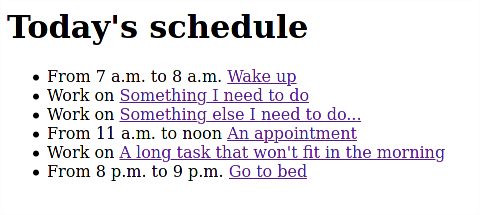
\includegraphics[width=0.8\linewidth]{Screenshots/example_schedule.png}
	\caption{What a day's schedule might look like}
	\label{fig:schedule1}
\end{figure}

\subsection{Stage 3 Testing}
There are two main things to test here:
\begin{samepage}
	\begin{itemize}
		\item that the scheduler produces timeslots in an expected way
		\item that the schedule view correctly displays the allocated timeslots
	\end{itemize}
\end{samepage}

Here are the tests I wrote for the scheduler:
\begin{lstlisting}[language=Python]
class SchedulerTests(TestCase):
    # Test that the scheduler assigns timeslots for all events and routines on a day
    def test_num_timeslots(self):
        # Specify number of events and routines.
        # These numbers should not be too large so that they can all fit in the one day.
        num_events = 10
        num_routines = 2

        # Create a bunch of events
        for i in range(num_events):
            event = Event(
                date=timezone.now().date(),
                start_time=dt.time(hour=i),
                end_time=dt.time(hour=i, minute=30),
            )
            # They need to be saved to the database so the scheduler can see them
            event.save()

        # Ditto for routines
        for i in range(num_routines):
            routine = Routine(
                day=timezone.now().date().weekday(),
                start_time=dt.time(hour=i + num_events),
                end_time=dt.time(hour=i + num_events, minute=30),
            )
            routine.save()

        # Run the scheduler
        update_schedule(timezone.now().date().weekday())

        # Check that the number of timeslots created is the total no. events and routines
        self.assertEquals(len(TimeSlot.objects.all()), num_events + num_routines)

    # A similar test, this time involving tasks
    def test_num_timeslots_with_tasks(self):
        # Specify number of events, routines and tasks.
        # These numbers should not be too large so that they can all fit in the one day.
        num_events = 10
        num_routines = 2
        num_tasks = 10

        # Create a bunch of events
        for i in range(num_events):
            event = Event(
                date=timezone.now().date(),
                start_time=dt.time(hour=i),
                end_time=dt.time(hour=i, minute=30),
            )
            # They need to be saved to the database so the scheduler can see them
            event.save()

        # Ditto for routines
        for i in range(num_routines):
            routine = Routine(
                day=timezone.now().date().weekday(),
                start_time=dt.time(hour=i + num_events),
                end_time=dt.time(hour=i + num_events, minute=30),
            )
            routine.save()

        # Ditto for tasks
        # I'll create all the tasks with time estimates of 0 so they should definitely be scheduled.
        for i in range(num_tasks):
            task = Task(time_estimate=dt.timedelta(minutes=0))
            task.save()

        # Run the scheduler
        update_schedule(timezone.now().date().weekday())

        # Check that the number of timeslots
        self.assertEquals(
            len(TimeSlot.objects.all()), num_events + num_routines + num_tasks
        )

    # Test that a task which is too long to be scheduled is not scheduled
    def test_unschedulable_task(self):
        # Have the first event of the day from 09:30 to 10:00
        first_event = Event(
            date=timezone.now().date(),
            start_time=dt.time(hour=9, minute=30),
            end_time=dt.time(hour=10),
        )
        first_event.save()

        # Have the last event of the day from 10:30 to 11:00
        last_event = Event(
            date=timezone.now().date(),
            start_time=dt.time(hour=10, minute=30),
            end_time=dt.time(hour=11),
        )
        last_event.save()

        # If the task is longer than 30 minutes, there won't be room to schedule it
        task = Task(time_estimate=dt.timedelta(hours=1))
        task.save()

        # Run the scheduler
        update_schedule(timezone.now().date().weekday())

        # There should only be two timeslots, as the task has not been scheduled
        self.assertEquals(len(TimeSlot.objects.all()), 2)

    # Given the test for no. timeslots with tasks, this is probably redundant,
    # but I'll do it anyway
    def test_schedulable_task(self):
        # Have the first event of the day from 09:30 to 10:00
        first_event = Event(
            date=timezone.now().date(),
            start_time=dt.time(hour=9, minute=30),
            end_time=dt.time(hour=10),
        )
        first_event.save()

        # Have the last event of the day from 10:30 to 11:00
        last_event = Event(
            date=timezone.now().date(),
            start_time=dt.time(hour=10, minute=30),
            end_time=dt.time(hour=11),
        )
        last_event.save()

        # If the task is shorter than 30 minutes, there is room to schedule it
        task = Task(time_estimate=dt.timedelta(minutes=10))
        task.save()

        # Run the scheduler
        update_schedule(timezone.now().date().weekday())

        # There should be three timeslots,
        # for the two events and the task
        self.assertEquals(len(TimeSlot.objects.all()), 3)

    # Test what happens when events have weird timings
    def test_end_before_start_event(self):
        # This event starts at 10:00 and finishes as 09:00
        invalid_event = Event(
            date=timezone.now().date(),
            start_time=dt.time(hour=10),
            end_time=dt.time(hour=9),
        )
        invalid_event.save()

        # Also make a valid event
        valid_event = Event(
            date=timezone.now().date(),
            start_time=dt.time(hour=11),
            end_time=dt.time(hour=12),
        )
        valid_event.save()

        # Run the scheduler
        update_schedule(timezone.now().date().weekday())

        # The scheduler shouldn't create a timeslot for the nonsensical event,
        # so there should only be one timeslot
        self.assertEquals(len(TimeSlot.objects.all()), 1)
\end{lstlisting}

I realised that I hadn't considered what would happen,
if the scheduler encountered an event which ended before it started.
In theory this should never happen because events are validated on creation,
requiring them to end after they start,
however the scheduler should be durable enough to deal with this just in case.
As I suspected,
the scheduler blindly creates a nonsensical timeslot for the event.
I considered how to do this,
and decided that best thing to do was to have the scheduler ignore such events.
This way is the least likely to produce unexpected behaviour.

The scheduler now checks that any timeslot it creates does not end before it starts.
Here is the affected piece of code:
\begin{lstlisting}[language=Python]
# Iterate over all the events and routines,
# creating corresponding time slots
for item in all_events:
    if isinstance(item, Event):
        ts = TimeSlot(
            date=date,
            start_time=item.get_start(),
            end_time=item.get_end(),
            associated_type="E",
            associated_event=item,
        )

    elif isinstance(item, Routine):
        ts = TimeSlot(
            date=date,
            start_time=item.get_start(),
            end_time=item.get_end(),
            associated_type="R",
            associated_routine=item,
        )

    # Before adding the timslot to the list,
    # check that it has sensible timings.
    # If it doesn't, we can just discard it.
    if ts.start_time <= ts.end_time:
        time_slots.append(ts)
\end{lstlisting}

With that added validation,
all tests now pass.
There were also no issues with the view:
it calls the scheduler correctly and displays all the timeslots correctly and in order.

\subsection{Stage 3 Review}
This section went a lot smoother than I had anticipated.
I think I can attribute that, primarily,
to having carefully worked through the logic of the scheduling algorithm beforehand.
This meant that my implementation worked almost flawlessly.

Now that stage 3 is complete it is possible to:
\begin{samepage}
	\begin{itemize}
		\item have the program automatically create your schedule for the day
		\item view the schedule,
		      containing all events and routines that day,
		      and tasks where the scheduler could find space
		\item link through to the detail view for any item in the schedule
	\end{itemize}
\end{samepage}

In other words,
it is now possible to create events, routines and tasks,
and have the program schedule tasks around events and routines -
the primary goal of the project!

\section{Stage 4: Time Tracking and User Statistics}
These are the two final components needed to complete the solution,
although in reality I find it most sensible to consider them as one module due to their interdependence.

\subsection{Tracking time spent on a task}
After some consideration,
I don't think it makes sense to implement the time tracking in the way originally conceived;
in a manner like Forest,
where time is tracked as a live counter in the program as you work.
This is because the problem trying to be solved is not really that of concentration on a task,
which is what Forest targets,
but rather of planning and keeping track of time.
So I think it would be more sensible to have the user enter the time they spend working on a task,
rather than compel them to use a timer built in to the program.
This would also avoid unhelpful situations which occur in a program like Forest,
where time has been spent working unrecorded,
and there is no way to rectify that.

I discussed this with SH,
here is the transcript.

\paragraph{Max} Hi SH.
As you're aware,
I'm nearing the end of the development of the product.
I've come to implementing the module for tracking time spent working on a task,
however I'm not sure if it's best to implement it as originally discussed.
\paragraph{SH} What do you mean?
\paragraph{Max} I originally designed the solution using an approach like Forest,
where time is tracked by a timer in the app as you are working.
However I think it might be better to instead have the user simply log the time they spend.
This means the user isn't forced into adopting the program into their workflow,
which may be an inconvenience,
and avoids situations where statistics are inaccurate due to the user forgetting to use the timer when doing work on a task,
since they can simply log the time spent working whenever they are finished.
\paragraph{SH} That's true,
but I suppose that means you can't force the user to stay concentrated on the task,
like Forest does?
\paragraph{Max} I suppose so,
however it was already impossible to be as restrictive as Forest due to being a web app,
rather than a native application.
Also, if the user wanted to enforce those restrictions on themself,
they could always use another app like Forest for that purpose,
essentially regulating their time,
while still using MyTime for planning and tracking their time.
\paragraph{SH} That's reasonable.
I suppose it's also helpful to keep the program's scope reasonable.
Ok, I'm happy with that change then.

So I went ahead with implementing the time tracking via a form on the task detail page,
which allows the user to record time that they've spent working on the task.
This required a new view to be written,
to be responsible for updating the time spent on a task,
and changes made to the existing task detail view and template,
to accommodate the new form.

The task detail now looks like this:
\begin{figure}[H]
	\centering
	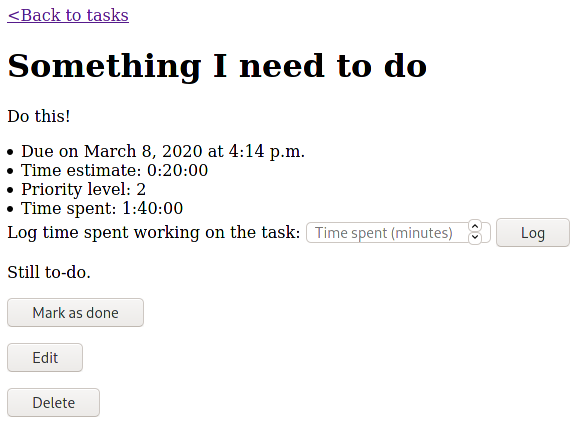
\includegraphics[width=\linewidth]{Screenshots/task_detail_with_time.png}
	\caption{Task detail with time logging form}
	\label{fig:task_detail2}
\end{figure}

Upon submitting the form with the ``log'' button,
the number in the form is sent to the task view,
which converts it to a Python timedelta object of the corresponding number of minutes,
and passed to the \texttt{alter\_time\_spent()} method of the task object.

\subsection{User Statistics}
In a slight change to the modular design outlined in figure \ref{fig:modular_design},
I decided to create a separate statistics-generation function,
\texttt{statistics.py}.
Although I could have handled generation of the statistics from the view,
I decided it would be best,
in terms of code readability and maintenance,
to make this separation.
Then, there are three components here:
the function for generating the statistics,
the view,
and the template.

As outlined in the design,
the usage statistics I want to be able to provide to the user are:
\begin{samepage}
	\begin{enumerate}
		\item Information on the timeliness of completion,
		      and accuracy of time estimation,
		      for recently completed tasks
		\item Overall number of tasks completed and time spent for the past day and week
		\item Overall statistics,
		      for all tasks,
		      of whether tasks are completed on time and within the time estimate
	\end{enumerate}
\end{samepage}

It made sense to further separate the function into two sub-procedures,
one for the generation of the specific statistics for the recent tasks,
and one for the generation of the overall statistics.
Here is the code for that,
it is moderately lengthy but quite straightforward:

\begin{lstlisting}[language=Python]
# Function for generating the overall statistics
def generate_overall_stats():
    # When this data is received by the view,
    # it will need to put it in the context dictionary,
    # so if we create a dictionary here is will be easy to copy. stats = {}

    # Here we'll do some queries to get various lists of tasks we'll need.
    # Note that we're listifying all the queries,
    # as Django provides Q objects,
    # which are a bit different.
    #
    # Tasks completed today:
    tasks_today = list(
        Task.objects.filter(
            done=True,
            completion_time__range=[timezone.now() - timedelta(days=1), timezone.now()],
        )
    )
    # Tasks completed this week:
    tasks_week = list(
        Task.objects.filter(
            done=True,
            completion_time__range=[timezone.now() - timedelta(days=7), timezone.now()],
        )
    )

    # Tasks completed on time:
    tasks_on_time = list(Task.objects.filter(done=True, completed_on_time=True))
    # Tasks completed within their time estimate
    tasks_in_time = list(Task.objects.filter(done=True, completed_in_time=True))

    # All completed tasks
    tasks_done = list(Task.objects.filter(done=True))

    # We simply look at the length of the respective lists,
    # to find out the number of tasks completed in the given timeframe.
    stats["num day"] = len(tasks_today)
    stats["num week"] = len(tasks_week)

    # Similarly we can sum the time_spent attributes of the tasks in each list,
    # to get the total time spent
    stats["time day"] = sum([task.time_spent for task in tasks_today], timedelta())
    stats["time week"] = sum([task.time_spent for task in tasks_week], timedelta())

    # Here we calculate the percentage, rounded to one decimal place,
    # of tasks completed on time and within their time estimate respectively
    stats["on time"] = round(100 * len(tasks_on_time) / len(tasks_done), 1)
    stats["in time"] = round(100 * len(tasks_in_time) / len(tasks_done), 1)

    # And return the dictionary
    return stats


# Function for generating the specific stats for given tasks
def generate_specific_stats(tasks):
    for task in tasks:
        # Create an offset-aware datetime object from the due date and due time,
        # for comparison with the completion datetime
        due = datetime.combine(task.due_date, task.due_time).replace(tzinfo=pytz.UTC)
        complete = task.completion_time

        # This is superflouous but makes the code look nicer
        spent = task.time_spent
        estimate = task.time_estimate

        # Get the difference between completion and due
        task.completion_delta = abs(due - complete)
        # Caculate the estimate accuracy as a percentage, rounded to 1 d.p.
        task.estimate_accuracy = round(abs(100 * ((spent / estimate) - 1)), 1)
\end{lstlisting}

These functions are both called by the statistics view,
which passes the data generated to the template to render.
Here is the result:
\begin{figure}[H]
	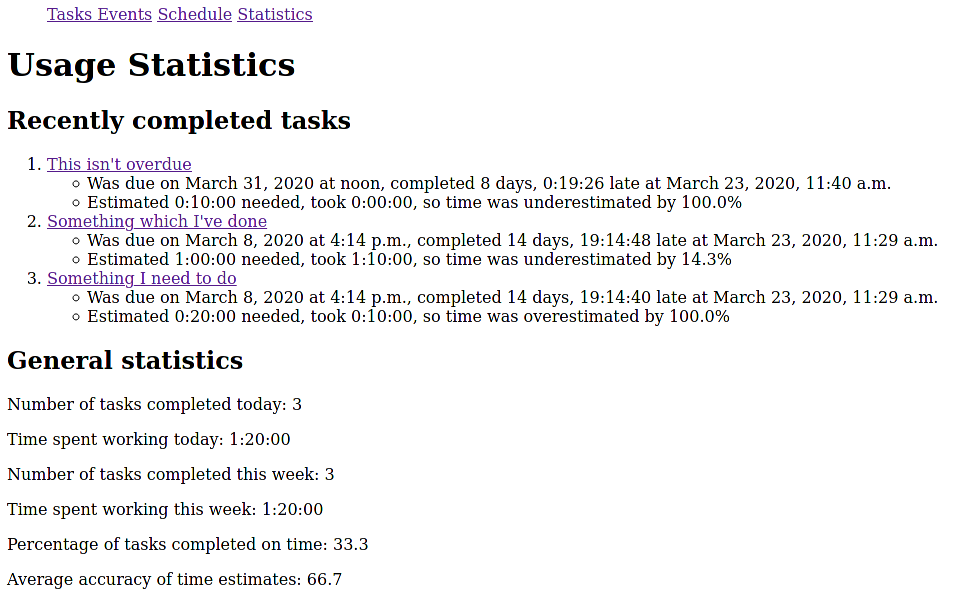
\includegraphics[width=\linewidth]{Screenshots/statistics.png}
	\caption{Screenshot of statistics page}
	\label{fig:statistics1}
\end{figure}

\subsection{Stage 4 Testing}
I wrote a number of tests to ascertain whether the statistics generator was working correctly.

Firstly, testing the function for generating stats on a per-task basis:
\begin{lstlisting}[language=Python]
class StatisticsTests(TestCase):
    # Test specific statistics generation
    def test_specific_stats(self):
        # This is just to make sure there are no unexpected small discretions in timings
        time = timezone.now()

        # Test large and small differences between due and completion
        late_one_day = Task(
            done=True,
            due_date=(time - dt.timedelta(days=1)).date(),
            due_time=time.time(),
            completion_time=time,
        )

        early_one_day = Task(
            done=True,
            due_date=time.date(),
            due_time=time.time(),
            completion_time=time + dt.timedelta(days=1),
        )

        late_one_minute = Task(
            done=True,
            due_date=time.date(),
            due_time=(time - dt.timedelta(minutes=1)).time(),
            completion_time=time,
        )

        early_one_minute = Task(
            done=True,
            due_date=time.date(),
            due_time=time.time(),
            completion_time=time + dt.timedelta(minutes=1),
        )

        exactly_due = Task(
            done=True, due_date=time.date(), due_time=time.time(), completion_time=time,
        )

        # Test large and small differences between time spent and estimated
        second_too_long = Task(
            done=True,
            time_estimate=dt.timedelta(seconds=10),
            time_spent=dt.timedelta(seconds=11),
        )

        second_too_short = Task(
            done=True,
            time_estimate=dt.timedelta(seconds=10),
            time_spent=dt.timedelta(seconds=9),
        )

        hour_too_long = Task(
            done=True,
            time_estimate=dt.timedelta(hours=10),
            time_spent=dt.timedelta(hours=11),
        )

        hour_too_short = Task(
            done=True,
            time_estimate=dt.timedelta(hours=10),
            time_spent=dt.timedelta(hours=9),
        )

        exactly_estimate = Task(
            done=True,
            time_estimate=dt.timedelta(minutes=10),
            time_spent=dt.timedelta(minutes=10),
        )

        tasks = [
            late_one_day,
            early_one_day,
            late_one_minute,
            early_one_minute,
            exactly_due,
            second_too_long,
            second_too_short,
            hour_too_long,
            hour_too_short,
            exactly_estimate,
        ]

        # Run the statistics generator on them
        generate_specific_stats(tasks)

        # All of them should be 10% off except for the exact ones
        self.assertEquals(late_one_day.completion_delta, 10)
        self.assertEquals(early_one_day.completion_delta, 10)
        self.assertEquals(late_one_minute.completion_delta, 10)
        self.assertEquals(early_one_minute.completion_delta, 10)

        self.assertEquals(second_too_long.estimate_accuracy, 10)
        self.assertEquals(second_too_short.estimate_accuracy, 10)
        self.assertEquals(hour_too_long.estimate_accuracy, 10)
        self.assertEquals(hour_too_short.estimate_accuracy, 10)

        self.assertEquals(exactly_due.completion_delta, 0)
        self.assertEquals(exactly_estimate.estimate_accuracy, 0)
\end{lstlisting}

Running these tests encountered the issue that,
in the statistics generator,
to find the accuracy of the time estimate I time spent by time estimate,
however time estimate defaults to 0,
so for the tasks without an estimate specified and error occurs.

Firstly,
I realised that the division should be the other way round,
as we are finding the error of the estimate from actual time spent,
not the other way around.
However,
time spent may also be 0,
so I also added in a check for this:
\begin{lstlisting}[language=Python]
# Caculate the estimate accuracy as a percentage, rounded to 1 d.p.
#
# Check that time spent is non-zero
if spent:
    task.estimate_accuracy = round(abs(100 * ((estimate / spent) - 1)), 1)
# If it's 0, then either the error is 0%, if the estimate was 0,
# or 100% if the estimate was anything else
elif estimate == timedelta(minutes=0):
    task.estimate_accuracy = 0
else:
    task.estimate_accuracy = 100
\end{lstlisting}

At this point I realised that I ought to have named \texttt{estimate\_accuracy},
\texttt{estimate\_error},
however I don't think this is a big enough issue to warrant refacoring.

Having corrected this I ran into a similar issue for tasks with a null completion time,
and made a similar correction:
\begin{lstlisting}[language=Python]
# Get the difference between completion and due,
# checking that the task does have a completion time
if complete:
    task.completion_delta = abs(due - complete)
else:
    task.completion_delta = timedelta(minutes=0)
\end{lstlisting}

Such an issue wouldn't arise in the typical operation of the program,
since it's impossible to mark a task as done without the completion time being assigned.
However this will catch any task that somehow is marked as done without a completion time,
because completion time is a field which is technically allowed to be null.

This resulted in a couple of tweaks to the existing tests and a couple new tests:
\begin{lstlisting}[language=Python]
class StatisticsTests(TestCase):
    # Test specific statistics generation
    def test_completion_delta_stats(self):
        # This is just to make sure there are no unexpected small discretions in timings
        time = timezone.now()

        # Test large and small differences between due and completion
        late_one_day = Task(
            done=True,
            due_date=(time - dt.timedelta(days=1)).date(),
            due_time=time.time(),
            completion_time=time,
        )

        early_one_day = Task(
            done=True,
            due_date=time.date(),
            due_time=time.time(),
            completion_time=time + dt.timedelta(days=1),
        )

        late_one_minute = Task(
            done=True,
            due_date=time.date(),
            due_time=(time - dt.timedelta(minutes=1)).time(),
            completion_time=time,
        )

        early_one_minute = Task(
            done=True,
            due_date=time.date(),
            due_time=time.time(),
            completion_time=time + dt.timedelta(minutes=1),
        )

        exactly_due = Task(
            done=True, due_date=time.date(), due_time=time.time(), completion_time=time,
        )

        tasks = [
            late_one_day,
            early_one_day,
            late_one_minute,
            early_one_minute,
            exactly_due,
        ]

        # Run the statistics generator on them
        generate_specific_stats(tasks)

        # Check that the values are what we would expect
        self.assertEquals(late_one_day.completion_delta, dt.timedelta(days=1))
        self.assertEquals(early_one_day.completion_delta, dt.timedelta(days=1))
        self.assertEquals(late_one_minute.completion_delta, dt.timedelta(minutes=1))
        self.assertEquals(early_one_minute.completion_delta, dt.timedelta(minutes=1))

        self.assertEquals(exactly_due.completion_delta, dt.timedelta(minutes=0))

    def test_estimate_accuracy_stats(self):
        # Test large and small differences between time spent and estimated
        second_too_long = Task(
            done=True,
            time_estimate=dt.timedelta(seconds=11),
            time_spent=dt.timedelta(seconds=10),
        )

        second_too_short = Task(
            done=True,
            time_estimate=dt.timedelta(seconds=9),
            time_spent=dt.timedelta(seconds=10),
        )

        hour_too_long = Task(
            done=True,
            time_estimate=dt.timedelta(hours=11),
            time_spent=dt.timedelta(hours=10),
        )

        hour_too_short = Task(
            done=True,
            time_estimate=dt.timedelta(hours=9),
            time_spent=dt.timedelta(hours=10),
        )

        exactly_estimate = Task(
            done=True,
            time_estimate=dt.timedelta(minutes=10),
            time_spent=dt.timedelta(minutes=10),
        )

        tasks = [
            second_too_long,
            second_too_short,
            hour_too_long,
            hour_too_short,
            exactly_estimate,
        ]

        # Run the stats generator
        generate_specific_stats(tasks)

        # Check the values
        self.assertEquals(second_too_long.estimate_accuracy, 10)
        self.assertEquals(second_too_short.estimate_accuracy, 10)
        self.assertEquals(hour_too_long.estimate_accuracy, 10)
        self.assertEquals(hour_too_short.estimate_accuracy, 10)
        self.assertEquals(exactly_estimate.estimate_accuracy, 0)

    # Test null values
    def test_specific_stats_null(self):
        time = timezone.now()

        # Create tasks with unusual attributes
        null_complete = Task(done=True, due_date=time.date(), due_time=time.time(),)

        zero_spent_zero_estimate = Task(done=True)

        zero_spent_nonzero_estimate = Task(
            done=True, time_estimate=dt.timedelta(minutes=10)
        )

        # Run the generator
        generate_specific_stats(
            [null_complete, zero_spent_zero_estimate, zero_spent_nonzero_estimate]
        )

        # Check the stats
        self.assertEquals(null_complete.completion_delta, dt.timedelta(minutes=0))
        self.assertEquals(zero_spent_zero_estimate.estimate_accuracy, 0)
        self.assertEquals(zero_spent_nonzero_estimate.estimate_accuracy, 100)
\end{lstlisting}

These tests all passed.

Then there were tests for the overall statistics generation:
\begin{lstlisting}[language=Python]
class GeneralStatisticsTests(TestCase):
    # Create n tasks today and n tasks yesterday
    def setup(self, n):
        # What's the time?
        time = timezone.now()
        yesterday = time - dt.timedelta(days=1)
        # Take precautionary measures
        Task.objects.all().delete()

        # Create a bunch of tasks, done today,
        # in less than estimated time and before their due date
        for i in range(n):
            Task(
                done=True,
                completed_on_time=True,
                completed_in_time=True,
                completion_time=time,
                time_spent=dt.timedelta(minutes=1),
            ).save()

        # Create a bunch of tasks, done yesterday,
        # in over the estimated time and overdue
        for i in range(n):
            Task(
                done=True,
                completed_on_time=False,
                completed_in_time=False,
                completion_time=yesterday,
                time_spent=dt.timedelta(minutes=1),
            ).save()

    def test_num_day(self):
        # Number of tasks
        n = 10
        # Run setup
        self.setup(n)

        # Generate stats
        stats = generate_overall_stats()

        # Check the number today
        self.assertEquals(stats["num day"], n)

    def test_num_week(self):
        # Number of tasks
        n = 10
        # Run setup
        self.setup(n)

        # Generate stats
        stats = generate_overall_stats()

        # Check the number this week
        self.assertEquals(stats["num week"], 2 * n)

    def test_time_day(self):
        # Number of tasks
        n = 10
        # Run setup
        self.setup(n)

        # Generate stats
        stats = generate_overall_stats()

        # Check the time spent today
        self.assertEquals(stats["time day"], timedelta(minutes=n))

    def test_time_week(self):
        # Number of tasks
        n = 10
        # Run setup
        self.setup(n)

        # Generate stats
        stats = generate_overall_stats()

        # Check the time spent this week
        self.assertEquals(stats["time week"], timedelta(minutes=2 * n))

    def test_on_time(self):
        # Number of tasks
        n = 10
        # Run setup
        self.setup(n)

        # Generate stats
        stats = generate_overall_stats()

        # Check the time spent today
        self.assertEquals(stats["on time"], 50)

    def test_in_time(self):
        # Number of tasks
        n = 10
        # Run setup
        self.setup(n)

        # Generate stats
        stats = generate_overall_stats()

        # Check the time spent today
        self.assertEquals(stats["in time"], 50)
\end{lstlisting}

These tests all passed:
this is unsurprising given the relatively simpler nature of the general stats generator.

\subsection{Stage 4 Review}
At this point at the end of development,
I was very familiar with the tools I was using,
so it was completed quite efficiently.
Likewise,
the tests were very thorough.

With stage 4 complete, it is now possible to:
\begin{samepage}
	\begin{itemize}
		\item generate various statistics about completed tasks,
		      both with respect to specific tasks and in general
		\item view these statistics
	\end{itemize}
\end{samepage}

And that's it -
The project is now fully functional.

\part{Evaluation}
\section{Functionality testing}
I sent my completed product to SH for testing.
After a week of use,
SH provided the following feedback on functionality:
\begin{samepage}
	\begin{itemize}
		\item The scheduler doesn't break up long tasks,
		      so when I create a task with a very long time estimate,
		      it often ends up not getting scheduled,
		      even if it is due soon and has high priority.
      \item It's annoying that you can't have events which at custom intervals,
        like daily or fortnightly,
        or copy routine events across multiple days -
        I have the same school day from Monday through Friday but I need to input it 5 times.
        Ditto for sleep schedule, it's the same most days and I have to input it many times.
      \item The task management works well,
        although I'd like more organisation options.
      \item I wish I could sync my calendar on my phone...
        I know that it was never planned but it's really annoying.
	\end{itemize}
\end{samepage}

See the section on limitations of the solution for analysis.

\section{Usability testing}
SH's feedback on usability:
\begin{samepage}
  \begin{itemize}
    \item I know about function over form but it's kind of basic looking.
    \item The buttons could be coloured and the navigation at the top is quite unattractive.
      It is good that they are there though,
      it helps to have a quicker workflow.
    \item Having a pile of buttons at the bottom of the screen doesn't look great,
      especially because they are sized differently.
      It would look more normal if they were next to each other rather than on top of each other.
  \end{itemize}
\end{samepage}

See the section on limitations of usability features for analysis.

\section{Evaluation of the solution against success criteria}
These were my success criteria at the start of the project:
\begin{samepage}
	\begin{enumerate}
		\item Store a list of the user's tasks
		\item Store the due date, priority, expected time needed, and other information
		      about each task
		\item Allow the user to add, edit and remove tasks from the list
		\item Record the successful completion of each task, time taken, and number of
		      breaks taken and display this information to the user in a useful manner
		\item Store information about the user's schedule,
		      including both regular and particular commitments
		\item Schedule time for the user to complete their tasks, according to the
		      user's schedule, task due date and task priority
		\item Display the tasks in their allocated time slots,
		      relative to the user's schedule
		\item Have a focus mode, which helps the user concentrate on the task at hand,
		      and incentivises the user to complete the task in a timely manner without
		      procrastination, using game-like aspects
		\item Track the time the user spends working on a task
		\item Provide feedback to the user about their completed tasks,
		      such as whether a task was completed on time and within the scheduled time slot,
		      and equivalent overall and average task statistics
		\item Be available on multiple platforms and devices
		\item Sync tasks between devices
	\end{enumerate}
\end{samepage}

I will go through these one by one,
explaining whether they have been met,
and showing how they have or have not been met.

\subsection*{Criterion 1}
Store a list of the user's tasks.

\paragraph{Status:}
Met.

\paragraph{Evidence:}
The program utilises a database;
within the database is held a table of tasks.

\subsection*{Criterion 2}
Store the due date, priority, expected time needed, and other information about each task

\paragraph{Status:}
Met.
\paragraph{Evidence:}
The table in the programs database has fields for
\begin{samepage}
	\begin{itemize}
		\item a due date
		\item a priority level
		\item the expected time needed
	\end{itemize}
\end{samepage}

It also has fields for
\begin{samepage}
	\begin{itemize}
		\item a title
		\item a more detailed description
		\item a due time
		\item a flag for whether or not the task is done
	\end{itemize}
\end{samepage}

And if the task is complete
\begin{samepage}
	\begin{itemize}
		\item the time at which the task was completed
		\item how long was spent working on the task
		\item whether it was completed on time
		\item whether it was completed within the estimated time
		\item the time delta between when it was completed and when it was due
		\item the percentage error from time spent to time estimated
	\end{itemize}
\end{samepage}

\subsection*{Criterion 3}
Allow the user to add, edit and remove tasks from the list.

\paragraph{Status:}
Met.

\paragraph{Evidence:}
The program provides a form through which a task can be created,
by entering a title,
description,
due date,
due time,
time estimate,
and priority level.
This can be can be accessed from a page showing the list of the user's tasks.

The program provides a form through which a task can be edited,
by entering a new title,
description,
due date,
due time,
time estimate,
and/or priority level.
This can be accessed from the page showing the details of a task,
which itself can be accessed from the aforementioned task list page.

The program provides a button to delete a task,
located on the aforementioned task detail page.

\subsection*{Criterion 4}
Record the successful completion of each task, time taken,
and number of breaks taken and display this information to the user in a useful manner.

\paragraph{Status:}
Partially met.

\paragraph{Evidence:}
Tasks may be marked as complete using buttons on the task list page or the task detail pages.
Time taken may be recorded using a form on the task detail page for each task.
It is not possible to record breaks taken.
Whether a task is complete or not is shown by it's categorisation on the task list page,
and it stated on the task's detail page.
The time spent on a task is shown on the task's detail page,
and further information comparing time taken to time estimated is shown on the statistics page.

This criterion could be met fully by either implementing the abandoned focus mode feature,
and allowing the user to pause the timer and tracking the number of times done so,
or by providing a form similar to the time spent form on the task detail page,
where the user can manually record breaks.

\subsection*{Criterion 5}
Store information about the user's schedule,
including both regular and particular commitments

\paragraph{Status:}
Met.

\paragraph{Evidence:}
The database has tables for storing data about events,
and routine (i.e. weekly recurring) events.
Specifically:
\begin{samepage}
	\begin{itemize}
		\item a title
		\item the date (event) or day (routine event) which they are on
		\item the start time
		\item the end time
	\end{itemize}
\end{samepage}

All the abilities for creation, updating, deletion, and viewing,
which are provided for tasks,
are also provided for events and routines.

\subsection*{Criterion 6}
Schedule time for the user to complete their tasks, according to the
user's schedule, task due date and task priority.

\paragraph{Status:}
Met.

\paragraph{Evidence:}
The program provides a function to schedule tasks,
between the user's various events and routine events.
It does so prioritising those tasks which are due sooner,
and which have higher priority.

\subsection*{Criterion 7}
Display the tasks in their allocated time slots,
relative to the user's schedule.

\paragraph{Status:}
Met.

\paragraph{Evidence:}
The program has a page showing the user's schedule for the day,
meaning the various events and routine events are shown in order with their timings,
and tasks are shown in their allocated slots between them.

\subsection*{Criterion 8}
Have a focus mode, which helps the user concentrate on the task at hand,
and incentivises the user to complete the task in a timely manner without
procrastination, using game-like aspects.

\paragraph{Status:}
Not met.

\paragraph{Evidence:}
As explained the third stage of development,
I abandoned this feature,
replacing it with manual time tracking through the task detail page.

This criterion could be met by implementing the feature as originally described in the design.
This would involve a focus mode page where a particular task could be selected to work on,
which included a timer which tracks time spent working,
and can be paused to record breaks.
On this page something could be shown which acts as a reward for continuously working,
such as city which grows over time,
as previously described,
and a ``high score'' showing the best city the user ever created
(being their longest continuous work session).

\subsection*{Criterion 9}
Track the time the user spends working on a task

\paragraph{Status:}
Met.

\paragraph{Evidence:}
This can be performed via a form on each task's detail page,
where time spent can be input and added to the current time spent for the task.

\subsection*{Criterion 10}
Provide feedback to the user about their completed tasks,
such as whether a task was completed on time and within the scheduled time slot,
and equivalent overall and average task statistics.

\paragraph{Status:}
Met.

\paragraph{Evidence:}
The program contains a function for calculating statistics about the user's completed tasks.
The statistics which may be calculated are:
\begin{samepage}
	\begin{itemize}
		\item the time delta between when a task was completed and when it was due,
		      for a specific task
		\item the percentage error of the estimated time from actual time taken,
		      for a specific task
		\item the number of tasks completed on a particular day
		\item the number of tasks completed in a particular week
		\item the total amount of time spent working on tasks on a particular day
		\item the total amount of time spent working on tasks in a particular week
		\item the percentage of all tasks completed on time
		\item the percentage of all tasks completed within their time estimate
	\end{itemize}
\end{samepage}

The program also displays the overall statistics,
alongside the specific statistics for the five most recently completed tasks,
on a statistics page.

\subsection*{Criterion 11}
Be available on multiple platforms and devices.

\paragraph{Status:}
Partially met.

\paragraph{Evidence:}
As the program is built as a webapp,
if hosted on the internet it can be accessed from any device or platform,
with access to the internet and compliant with internet standards.
However, I do not have access to a server which could host the program.

This criterion could be met by deploying running the program on a server with a domain,
so that it can be accessed on the world wide web.

\subsection*{Criterion 12}
Sync tasks between devices.

\paragraph{Status:}
Partially met.

\paragraph{Evidence:}
Refer to criterion 11.

\section{Evaluation of usability features}
I implemented all the usability features set out.
\begin{samepage}
	\begin{itemize}
		\item Any reference to a task, event or routine contains a link to that items detail view.
		\item Buttons to toggle the todo/done status are present for all tasks,
		      both on the index and in their detail view.
		\item All pages have a navigation bar including links to the task list,
		      event list,
		      scheduler,
		      and statistics pages.
	\end{itemize}
\end{samepage}

Note also that the todo/done buttons change their text depending on the current status of the task,
so when the task is todo the button will read ``Mark as done'',
and when it is done the button will read ``Mark as todo''.

Here is a screenshot of these features in action:
\begin{figure}[H]
	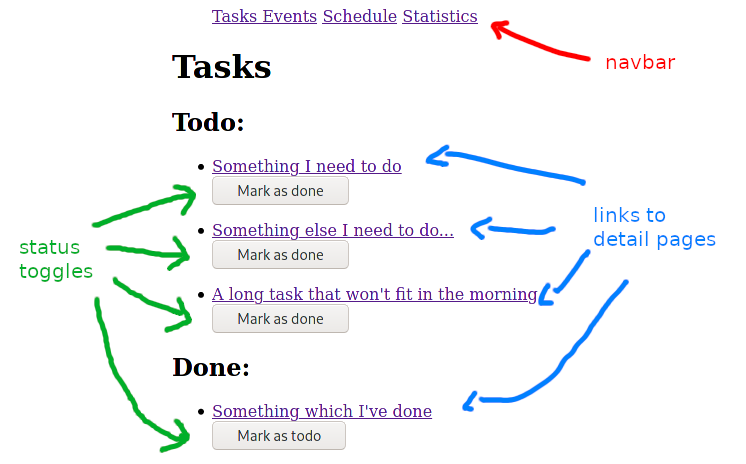
\includegraphics[width=\linewidth]{Screenshots/task_index_usability.png}
	\caption{Screenshot of task index showing most usability features}
	\label{fig:task_index_usability}
\end{figure}

\subsection{Limitations of usability features}
The main limitation with my usability features is that they are quite unattractive.
It could be helpful, for example,
for the status toggle buttons to change colour,
according to whether they will change to todo or done,
and the navigation bar looks very basic as well.
The links through to the task detail could also look nicer,
or possibly be replaced with buttons.
In general it would be nicer for buttons to be colour coded and arranged more carefully,
in particular,
the stack of three buttons at the bottom of the task detail page looks quite bad.

The issue here is that I simply didn't dedicate enough time to the user interface.
In terms of functionality it's all there,
and everything is clearly labelled,
but nothing about it is attractive or good looking.
With some more time,
I could have improved the situation through the use of CSS.

\section{Limitations of the solution}
The biggest limitation of my solution is the inflexibility of the scheduler.
Particularly,
it would be very useful if it were able to break tasks down into smaller chunks,
in case a whole task cannot be fit in a particular time slot,
or to provide the user with breaks,
or to alternate between different tasks,
according to user preference.
Without such an ability,
the program is only suited to scheduling the sort of tasks that can be completed in one go.
Furthermore,
the program always attempts to schedule tasks in free time,
even if, for example,
the task with which the space is filled is not due for a very long time.
In short,
the scheduling algorithm I use is not very intelligent,
and doesn't make best use of the information available to it.

Additionally,
it is currently only possible for the user to view their schedule for the day.
User's might like to, at least, view their schedule for the next week.
The scheduler is also not aware of whether or not the user completes their tasks as allocated,
so cannot,
for example,
reschedule a task the user failed to complete for later in the day -
it can only reschedule it tomorrow.
This inflexibility limits the usefulness of the solution as it currently is.

Furthermore,
despite acting as a task manager and calendar,
the solution does not contain features typical of such programs.
Task categorisation is absent,
as is the ability to have events which occur anything other than weekly.
This limits the efficacy of the solution in performing those roles.

The solution is also limited in the way it shows statistics about completed tasks.
The user can't access specific statistics beyond a set number of recently completed tasks,
and can't access statistics for particular days or weeks except the current day and current week.
Access to such information may be desired by the user.

Overall,
the solution suffers from a problem of scope -
because the scope was too broad,
every component is in some sense limited,
and not developed to as full an extent as it could have been.
This is the case despite a fairly significant feature,
the focus mode,
having been cut.
If I had not needed to develop task management and calendaring functionality,
a lot more time could have been devoted to developing the scheduler,
and providing flexibility and customisation that would have made it much more useful.
The same can be said for the statistics tracking component.

\subsection{Potential solutions to these limitations}
With regard to the scheduler,
more time would allow the development of a better algorithm.
It would be easy to drop in a new algorithm once developed,
due to the modular nature of the solution.

In terms of task management and calendaring,
I think the task management could be fleshed out with more development time -
providing categorisation of tasks would bring this mostly up to standard,
and the ability to add attachments to tasks is also a common feature.
However,
I think the best way forward to calendaring would be to scrap the current implementation,
replacing it with the ability to sync with external calendars,
such as Google Calendar,
Apple Calendar,
or CalDAV.
Good calendar solutions already exist which most user's will use,
so it is better not to force the user to switch from their existing calendar,
which probably integrates better with their devices and other services such as email.

The statistics could also be improved by providing the user with task-specific stats on the task detail pages,
and by giving options on the statistics page to view statistics for other days and weeks in the past.

\label{page:the_end}
\end{document}

% LocalWords:  MyTime Evernote Trello Todoist subtasks TimeSlot tuples
